\documentclass[a4paper]{book}

\usepackage{draftwatermark}
\SetWatermarkText{Draft}
\SetWatermarkColor[gray]{0.9}

\usepackage[utf8]{inputenc}
\usepackage[T1]{fontenc}

\usepackage{titlesec, blindtext, xcolor}
\definecolor{gray75}{gray}{0.75}
\definecolor{base00}{HTML}{fafafa}
\definecolor{base01}{HTML}{d4d4d4}
\definecolor{base02}{HTML}{abacae}
\definecolor{base03}{HTML}{7e8087}
\definecolor{base04}{HTML}{555761}
\definecolor{base05}{HTML}{333333}
\definecolor{base06}{HTML}{4d4d4d}
\definecolor{base07}{HTML}{666666}
\definecolor{base08}{HTML}{a10705}
\definecolor{base09}{HTML}{0d52bf}
\definecolor{base0A}{HTML}{cc3b02}
\definecolor{base0B}{HTML}{57392d}
\definecolor{base0C}{HTML}{d48e15}
\definecolor{base0D}{HTML}{3a9104}
\definecolor{base0E}{HTML}{7239b3}
\definecolor{base0F}{HTML}{667885}

\newcommand{\hsp}{\hspace{10pt}}
\titleformat{\chapter}[hang]{\Huge\bfseries}{\textcolor{base02}{\thechapter }\hsp}{0pt}{\Huge\bfseries}
\titleformat{\section}[hang]{\Large\bfseries}{\textcolor{base01}{\thesection}\hsp}{0pt}{\Large\bfseries}
\titleformat{\subsection}[hang]{\large\bfseries}{\textcolor{base01}{\thesubsection}\hsp}{0pt}{\large\bfseries}

\usepackage[american]{babel}
\usepackage{csquotes}
\usepackage[style=apa,sortcites=true,sorting=nyt,backend=biber]{biblatex}
\DeclareLanguageMapping{american}{american-apa}
\addbibresource{references.bib}

% Essentials
\usepackage{tabularx}
\usepackage{supertabular}
\usepackage{graphicx}
\usepackage{subcaption}
\usepackage{lscape}
\usepackage[ruled]{algorithm2e}

% Typography
\usepackage{palatino}
\usepackage{fontenc}

% Links
\usepackage[colorlinks=true, citecolor=base08, linkcolor=base08, urlcolor=base08]{hyperref}

% Math stuff
\usepackage{amsmath}
\usepackage{amssymb}
\usepackage{amstext}
\usepackage{bm}

% Drawings
\usepackage{tikz}
\usetikzlibrary{arrows.meta, fit, positioning, shapes}
\newcommand{\empt}[2]{$#1^{\langle #2 \rangle}$}

%% Drawing plots from PGFPlots
\usepackage{pgfplots}
\pgfplotsset{compat=newest}
\usepgfplotslibrary{groupplots}
\usepgfplotslibrary{dateplot}

\tikzset{
    neuron/.style={
        circle, draw, thick,
        inner sep=0pt,
        minimum size=3.0em,
        node distance=4em
    },
    io/.style={
        neuron,
        fill=base01
    },
    conn/.style={
        thick,
        -{Straight Barb[angle=60:2pt 3]},
    },
    connl/.style={
        thick,
        {Straight Barb[angle=60:2pt 3]}-,
    },
    prod/.style={circle, draw, thick, inner sep=0pt},
    ct/.style={circle, draw, inner sep=0pt, ultra thick,
		minimum size=3.0em, node distance=4em},
    ft/.style={circle, draw, thick, minimum width=8mm, inner sep=1pt},
    filter/.style={circle, draw, thick, minimum width=7mm, inner sep=1pt,
		path picture={
			\draw[thick, rounded corners] (path picture bounding box.center)--++(65:2mm)--++(0:1mm);
			\draw[thick, rounded corners] (path picture bounding box.center)--++(245:2mm)--++(180:1mm);}},
}

% Commands
\DeclareMathOperator*{\argmin}{arg\,min}
\DeclareMathOperator*{\argmax}{arg\,max}

\begin{document}

\begin{titlepage}
    \begin{center}
        \huge\textbf{Composing like a human:} \\
        \Large\textbf{Adapting generative networks to few-shot learning in the musical domain}
        \normalsize

        \vspace{1cm}

        \textbf{Tudor Paisa}\\
        Student Number: 2019551 \\
        Administration Number: 315146\\
        t.paisa@tilburguniversity.edu\\

        \vspace{1cm}
        \textsc{Thesis submitted in partial fulfillment\\
        of the requirements for the degree of\\
        Master of Science in Data Science and Society,\\
        at the School of Humanities and Digital Sciences\\
        of Tilburg University\\}

        \vspace{2cm}
        Thesis Committee:\\
        Dr. Menno van Zaanen\\
        Dr. Martin Atzmueller\\
        \vfill

        Tilburg University\\
        School of Humanities and Digital Sciences\\
        Department of Cognitive Science \& Artificial Intelligence\\
        Tilburg, The Netherlands\\
        \today
 
    \end{center}
\end{titlepage}

\chapter*{Abstract}
    Lorem Ipsum

\tableofcontents

\chapter{A hazy shade of winter}
%Simon and Garfunkel - A hazy shade of winter

Over the past sixty years, Artificial Neural Networks (ANNs) have experienced several popularity cycles noted in the literature by extensive publicity of over-inflated expectations with regards to the promises of connectionism (the field of science that tries to explain mental phenomena with the help of ANNs) \parencite{minsky_perceptrons_1988, knight_ai_2016, nilsson_speed_2009}. More specifically, it promised that a system could learn to do anything it was programmed to do \parencite{minsky_perceptrons_1988}. However, each wave of praise was followed by a mass of public disappointment, criticism, and funding cuts \parencite[e.g.,][]{lighthill_artificial_1972}. These upturns and downturns of the field of connectionism - or more generally A.I. - are now known in the literature as the A.I. winters \parencite{nilsson_speed_2009}.

The recent revival of ANNs under the brand of Deep Learning (DL) has brought new ways to tackle Machine Learning problems - most notably in the context of classification (but also regression, although less popular; see \cite{lecun_deep_2015} for several examples). In addition, with the advent of chatbots \parencite{dale_return_2016}, voice-activated personal assistants \parencite{xiong_microsoft_2018}, and general-purpose A.I. systems \parencite{vinyals_starcraft_2017}, DL introduced new frontiers in artificial intelligence research.

Broadly speaking, DL as a field, promises to solve tasks which are easily (intuitively) performed by people, but hard to formalize \parencite[e.g., recognizing faces or spoken word;][]{goodfellow_deep_2016}. The solution comprises of enabling computers to learn from experience and understand the world through the discovery of hierarchical relationships between concepts \parencite{lecun_deep_2015}. This way, there is no need for manual input on the sort of knowledge that the computer needs \parencite{goodfellow_deep_2016}. A more simplistic and concise interpretation of DL would be to see it as a statistical technique for identifying patterns in sample data using large (deep) ANNs \parencite{marcus_deep_2018}.

The reasons for presenting these facts will be clarified bit-by-bit throughout this chapter (Section \ref{sec:thesis_goal} provides a concrete explanation) however, a terse argumentation is that progress towards general A.I. systems is marked by scant explorations of ANNs outside of the classification task, and even more so when trying to overcome some of their shortcomings, such as being highly reliant on massive amounts of data.
% NOTE: Maybe I was too harsh?

\section{Strange Fruit}\label{sec:no_disc}
% Billie Holiday - Strange Fruit

Typically, in a neural network, data samples go through a set of input units (that might represent pixels, word embeddings, etc.), then through multiple hidden layers, each with a given number of nodes, and reaching the output units where the answer is given \parencite{marcus_deep_2018}. An overwhelming majority of experiments with ANNs involve discriminative models \parencite{goodfellow_generative_2014}, where the goal is to assign high-dimensional inputs to a single class label \parencite[such as an animal or piece of furniture;][]{zhang_character-level_2015, krizhevsky_imagenet_2012}. However, other possible applications of DL models include (but are not limited to): regression \parencite{qiu_ensemble_2014}, data compression \parencite{cheng_deep_2018}, and generating new data points \parencite{graves_generating_2013}.

The last point mentioned above is particularly interesting not because it has gained a lot of traction in recent years, but because of its potential to assist the scientific community as well as the general population. Borrowing the analogy from \textcite{goodfellow_nips_2016}, one might wonder what is the value of studying generative models. If, for instance, we are dealing with images, such a framework would merely generate more images for us (something which the Internet as no shortage of). This sort of worldview, however, would only limit these systems from their full capacity; aside from the obvious use case, generative networks could also be used for simulating possible futures - such as for scheduling and planning \parencite{finn_deep_2016} -, for providing predictions to missing data, or for enabling work on multi-modal outputs, where a single input may have more than one correct answer \parencite{goodfellow_nips_2016}.

Regardless, successes in generative models have been either scarce or unattractive, with Fully Visible Belief Networks \parencite{frey_does_1996} being the most suitable (and popular) method for the longest run. Given the age and - alleged - popularity, a valid question to ask is why things haven't moved that much since then. As it turn out, this method requires generating one sample at a time (ramping up the cost of the process to $O(n)$). Coupled with the fact that the computation is done through a neural network, creating $n$ samples requires a substantial amount of time \parencite{goodfellow_nips_2016}. This discussion is not exhaustive; for a comprehensive list of various generative approaches and their downsides, refer to \textcite{goodfellow_nips_2016}.
%Variational Autoencoders \parencite{kingma_auto-encoding_2013} are another popular method that is used for this sort of task. Their main drawback however, is that when a weak approximation of a prior or posterior distribution of the data is used, the model might learn something other than the true data distribution \parencite{goodfellow_nips_2016}.

The discovery of Generative Adversarial Networks \parencite[GANs;][]{goodfellow_generative_2014} has leapfrogged the state of developments in this field. Besides countering the drawbacks outlined above, they have been particularly successful at a variety of tasks such as image super-resolution \parencite[; see Figure \ref{fig:srgan}]{ledig_photo-realistic_2016}, style-based image generation \parencite{karras_style-based_2018}, or image-to-image translation \parencite[such as converting a satellite image into a map, or a sketch into a photorealistic image;][;see Figure \ref{fig:pix2pix}]{isola_image--image_2016}.

Similarly, and although not as popular, Recurrent Neural Networks (RNNs) have been successful at various generative tasks \parencite{jenal_rnn-based_2019, ICML2011Sutskever_524}. The reason is because RNNs contain a high-dimensional hidden state which allows them to remember and predict from previous inputs \parencite{ICML2011Sutskever_524}. This made them great candidates for predicting sequences \parencite{graves_generating_2013} of text or characters, where the input at $t_0$ might be influenced by prior input at $t_{-1}$, $t_{-2}$, etc. \parencite{fan_tts_2014}. That being said, Long Short-Term Memory networks \parencite[LSTM;][]{hochreiter_long_1997} - a variant of RNNs - have been purpose-built with memory cells which permit better storing and accessing of information. This design decision variant of the recurrent network good candidates for generating sequences with long-term dependencies \parencite{graves_generating_2013}.

\begin{figure}[t]
    \centering
    \begin{subfigure}{.24\linewidth}
        
\includegraphics[width=\linewidth]{images/comic_HR.jpg}
        \caption{original}
        \label{fig:srgan_orig}
    \end{subfigure}
    \begin{subfigure}{.24\linewidth}
        
\includegraphics[width=\linewidth]{images/comic_SRF_4_bicubic.jpg}
        \caption{bicubic}
        \label{fig:srgan_bicubic}
    \end{subfigure}
    \begin{subfigure}{.24\linewidth}
        
\includegraphics[width=\linewidth]{images/comic_SRResNet-MSE.jpg}
        \caption{SRResNet}
        \label{fig:srgan_srresnet}
    \end{subfigure}
    \begin{subfigure}{.24\linewidth}
        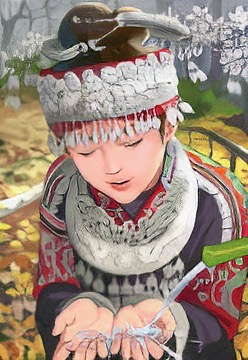
\includegraphics[width=\linewidth]{images/comic_SRGAN-VGG54.jpg}
        \caption{SRGAN}
        \label{fig:srgan_srgan}
    \end{subfigure}

    \caption{Example of single-image super-resolution results that highlight the advantages of a GAN. The original high-resolution image (\ref{fig:srgan_orig}) has been downsampled to make a low-resolution image. The results of bicubic interpolation (\ref{fig:srgan_bicubic}) can be seen in the second image, followed by the results of SRResNet (\ref{fig:srgan_srresnet}), a neural network trained on mean squared error. Lastly, the results of SRGAN can be seen in the final image (\ref{fig:srgan_srgan}). Figure adapted from \textcite{ledig_photo-realistic_2016}.}
    \label{fig:srgan}
\end{figure}

\begin{figure}[t]
    \centering
    \begin{tabular}{ccc}
    Input & Ground Truth & Output \\
    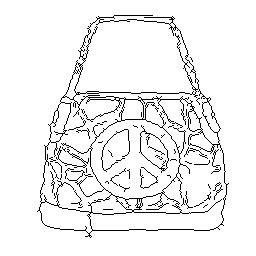
\includegraphics[width=.15\linewidth]{images/handbags_edges_lotsofresults_latex/input_106_AB.jpg} &
    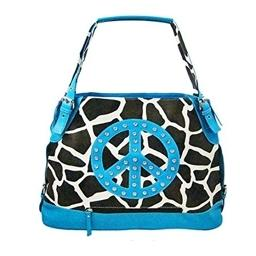
\includegraphics[width=.15\linewidth]{images/handbags_edges_lotsofresults_latex/gt_106_AB.jpg} &
    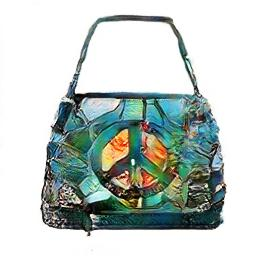
\includegraphics[width=.15\linewidth]{images/handbags_edges_lotsofresults_latex/L1cGAN_106_AB.jpg} \\
    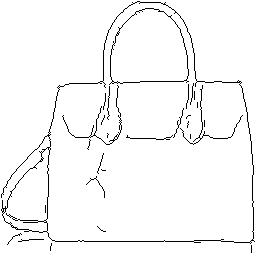
\includegraphics[width=.15\linewidth]{images/handbags_edges_lotsofresults_latex/input_12_AB.jpg} &
    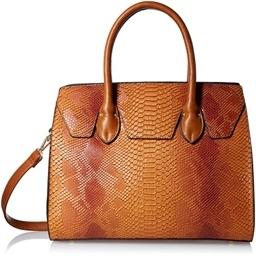
\includegraphics[width=.15\linewidth]{images/handbags_edges_lotsofresults_latex/gt_12_AB.jpg} &
    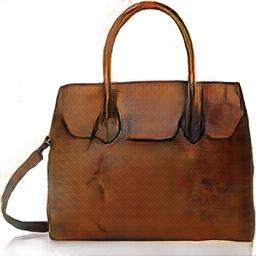
\includegraphics[width=.15\linewidth]{images/handbags_edges_lotsofresults_latex/L1cGAN_12_AB.jpg} \\
    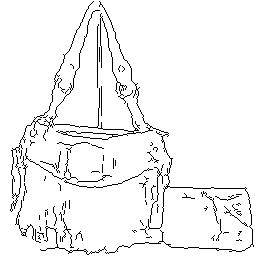
\includegraphics[width=.15\linewidth]{images/handbags_edges_lotsofresults_latex/input_130_AB.jpg} &
    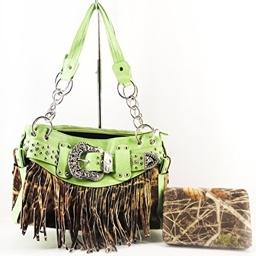
\includegraphics[width=.15\linewidth]{images/handbags_edges_lotsofresults_latex/gt_130_AB.jpg} &
    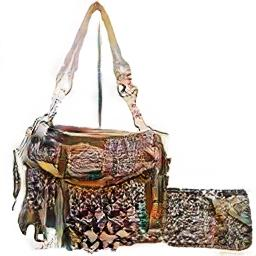
\includegraphics[width=.15\linewidth]{images/handbags_edges_lotsofresults_latex/L1cGAN_130_AB.jpg} \\
    \end{tabular}
    \caption{\textcite{isola_image--image_2016} coined the term image-to-image translation where an input image is transformed into a revisualization of the original input. This figures illustrates how an outline of a purse (leftmost column) is transformed into a colored photorealistic version of it (rightmost column). In the middle we have the ground truth: the real image of the purse. Figure adapted from \textcite{isola_image--image_2016}.}
    \label{fig:pix2pix}
\end{figure}

Having said all of these, the majority of developments with generative models lie in the field of Computer Vision. But that is not to say that we can generate only images. Generative models have been applied with varying degrees of success also in Natural Language Processing - where the scope was to generate high-quality text with sufficient diversity \parencite[e.g.,][]{yu_seqgan_2016, chen_adversarial_2018}. Less explored, but still successful, have been the efforts in generating music \parencite[e.g.,][]{mogren_c-rnn-gan_2016, dong_musegan_2017}. Herein lies the scope of this paper. Given such minimal explorations into generating music, we evaluated the samples generated by a GAN \parencite{mogren_c-rnn-gan_2016} and a LSTM network \parencite{oore_this_2018} trained under the constraints imposed by few-shot learning (Section \ref{sec:hungry}) against a baseline model proposed by \textcite{larochelle_few-shot_2017}. To reiterate, a full explanation of the purpose of the paper is provided in Section \ref{sec:thesis_goal}.

\section{I want it all}\label{sec:hungry}
% Queen - I want it all

DL models usually rely on a procedure called stochastic gradient descent (SGD) which implies computing an output and an error for a given input vector, followed by calculating the input's average gradient and adjusting the network's parameters in a manner that minimizes the error \parencite{lecun_deep_2015}. \textcite{ravi_optimization_2016} argue that the iterative nature of gradient-optimization algorithms does not allow them to perform well under the constraint of a set number of updates over few examples. In particular, when faced with non-convex optimization problems, DL algorithms do not guarantee convergence within a reasonable amount of time. In addition, they also emphasize that for each new problem (e.g., new dataset), the model needs to reinitialize with a new set of random parameters. Ultimately, this hurts the network's ability to converge to a good solution when constrained by a limited number of updates \parencite{ravi_optimization_2016}. Thus they lay out two clear drawbacks of DL models: "data-hunger", and inability to perform separate tasks.

A clear outcome from solving these issues would be that DL models are easier to train (less data) as well as multifunctional. Nonetheless, this list is not exhaustive. There is also fact that humans have the ability to generalize after one (or few) example(s) of a given object \parencite{vinyals_matching_2016, chen_closer_2018, ravi_optimization_2016} - something which DL models tend to lack. Moreover, there are many fields where the data exhibits a large number of classes, with few examples per class. Bridging the gap between human-type learning and current learning architectures would allow a system to do a proper job at capturing and generalizing information from sparse data \parencite{ravi_optimization_2016, larochelle_few-shot_2017}. This has motivated a series of explorations in the direction of "few-shot" learning (i.e., learning a class from a few examples) or more broadly, into the field of "meta-learning" \parencite[learning to learn in hopes of generalizing to new tasks;][]{chen_closer_2018, vinyals_matching_2016, zhang_metagan_2018}.

In spite of its proposed benefits, developments and experiments with few-shot learning are still scarce \parencite{larochelle_few-shot_2017}. Moreover, evaluations are largely concentrated on image data \parencite[see][]{lake_omniglot_2019, clouatre_figr_2019, vinyals_matching_2016, chen_closer_2018, ravi_optimization_2016}. Having said that, few-shot experiments with generative networks are even less frequent; \textcite{clouatre_figr_2019}, \textcite{dong_musegan_2017} and \textcite{zhang_metagan_2018} being some of the early (and few) explorers in this direction.

\section{Composing like a human} \label{sec:thesis_goal}

At the time of writing, generative models and meta-learning are two exciting areas of research the intersection of which could be quite promising. However, to the knowledge of the researcher, no experiments which combine the both of them have been conducted in the musical domain. Thus, this paper examined the extent to which generative models can create novel and qualitative samples of music under the constraints posed by few-shot learning. In other words, it sought to evaluate the degree to which generative models can create novel and high-fidelity samples when training data is scarce. To avoid any ambiguity, novel is used here as new (i.e., not in the training set), and qualitative as consistent with common scales and structurally diverse (combines chord structures with single-note sequences and is not restricted to only a few notes).

This research will evaluate the generated samples of two state-of-the-art generative models (C-RNN-GAN of \cite{mogren_c-rnn-gan_2016} and Performance-RNN of \cite{oore_this_2018}) that have been trained under a meta-learning framework, Reptile \parencite{nichol_first-order_2018}, with a limited number of songs. The performances of these two models were compared to the baseline proposed by \textcite{larochelle_few-shot_2017} and to recorded performances played by expert piano players at the International e-Piano Competition \parencite{university_of_minnesota_international_2019}.

In other words, this study sought to answer the following research questions:

\begin{itemize}
    \item To what extent is the music created by a few-shot generative model comparable to the music of a generative model that is trained on the entire dataset?
    \item To what extent is the music created by a few-shot generative model comparable to real music?
\end{itemize}

The following chapters will discuss more about generative models, meta-learning, and some of the models and algorithms involved in this paper (Chapter \ref{chap:theoretical_framework}), followed by a detailed description of the setup of the experiments (Chapter \ref{chap:methods}), and the results obtained from them (Chapter \ref{chap:results}). Finally, Chapter \ref{chap:discussion} closes with a discussion of the results and limitations of the experimental setup, whereas Chapter \ref{chap:conclusion} concludes the findings of this paper.

\chapter{Related Work}\label{chap:theoretical_framework}

This chapter takes a deep-dive into the fields of meta-learning and generative networks in order to highlight their current state of affairs. This will lay the groundwork for the experiments detailed in Chapter \ref{chap:methods}. Section \ref{sec:rnn} will present the principal network architecture of this paper, the recurrent neural network, and argument for its use as the foundation of a generative network. Section \ref{sec:generative} will introduce Generative Adversarial Networks, a training method build specifically for the task, whereas Section \ref{sec:learn2learn} will formally introduce meta-learning and some state-of-the-art approaches. 

\section{Recurrent Neural Networks} \label{sec:rnn}

In a standard ANN, the data traverses the network through the input layer, to the hidden layers, and finally the output layer; this setup is generally known as a feedforward neural network \parencite[Figure \ref{fig:feedforward_net};][]{graves_supervised_2012}. Broadly speaking, this type of network is defined by the fact that its connections do not form cycles. If however we relax this condition, we arrive at a recurrent neural network \parencite[Figure \ref{fig:rnn_folded};][]{rumelhart_learning_1986}: a family of neural networks specifically designed for processing sequential data \parencite{goodfellow_deep_2016}.

For transparency, it should be noted that it is possible to use a feedforward architecture, specifically a one-dimensional Convolutional Neural Network, with sequential data, where the convolution forms the basis of a time-delay neural network. Unfortunately, the output of such a system would be a function of a small number of neighbouring data points \parencite[such as the last and the next three notes in a song;][]{goodfellow_deep_2016}. Despite that, a system that uses convolution would quickly reach its limitation in the musical domain. Here, knowledge of the notes played from the beginning of the song is needed, meaning that we need an architecture that is able to account for long-term dependencies - which brings us back to the RNN.

The information passes through the RNN in a similar manner to the feedforward network except that the activations which arrive at the hidden layer are from the current external input and hidden activations from the previous timestep. It should be noted that the parameters of a recurrent network (weights) are shared across different timesteps \parencite{graves_supervised_2012}. This allows extending (and applying) the model to data points of different lengths whilst generalizing across all of them \parencite{goodfellow_deep_2016}. To place this into perspective, a feedforward network would require separate parameters for each input feature, at each position.

Thus, a formal definition of the network's forward pass would be
\begin{equation}
    h^t = f(h^{t-1}; x^t; \theta) \label{eq:rnn_hidden}
\end{equation}
where $h^t$ is the state of the hidden layer at time $t$, $x^t$ is the input at time $t$, and $\theta$ the model parameters.

The backward pass in a RNN is similar to that of a feedforward network: given the partial derivatives of a differentiable loss function $\mathcal{L}$ we calculate the derivatives with respect to the network's weights \parencite{graves_supervised_2012}. In this setting, a popular algorithm is called backpropagation through time \parencite[BPTT;][]{werbos_backpropagation_1990} which consists of repeated applications of the chain rule. The difference between standard backpropagation and BPTT is that the loss function depends on the activation of the hidden layer through its influence on the output layer as well as its influence on the hidden layer at the next timestep \parencite{graves_supervised_2012}.

Equation \ref{eq:rnn_hidden} can be drawn as in Figure \ref{fig:rnn_folded}: input sequences $x$ are mapped to a hidden layer $h$ and an output $y$, with the state of the hidden layer at time $t$ feeding back into itself with a time delay of $1$. In other words, the state of $h_t$ will influence the decision of the recurrent layer at time $t+1$. Another way to illustrate this is to unfold the computational graph such that each component of the network is represented by different variables per step, as in Figure \ref{fig:rnn_unfolded}.

The reason why these notions have been introduced is to be able to bring up the following point. As good as standard RNNs are - in theory - at accessing contextual information when mapping input sequences to output sequences, the range of contexts that can be accessed in a standard RNN architecture is in practice quite limited \parencite{graves_supervised_2012}. \textcite{hochreiter_long_1997} outlines two problems caused by BPTT: the error signals flowing backwards in time tend to either (1) blow up or (2) vanish. As such, the Long Short-Term Memory network has been proposed, a recurrent architecture designed to overcome these issues \parencite{hochreiter_long_1997}.

\begin{figure}[t]
    \centering
    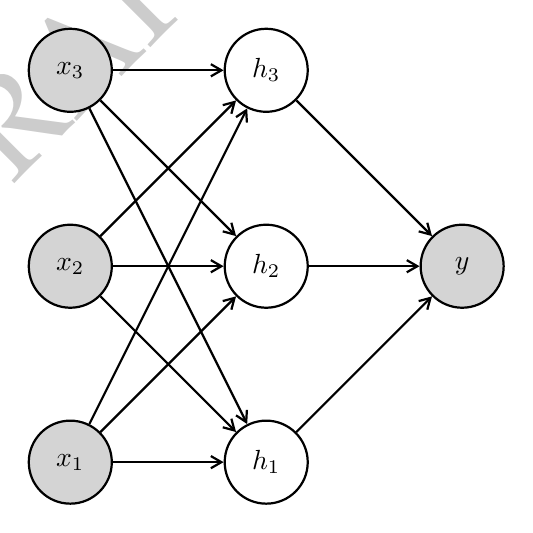
\begin{tikzpicture}
        \node[io] (x1) {$x_1$};
        \node[io, above=4em of x1] (x2) {$x_2$};
        \node[io, above=4em of x2] (x3) {$x_3$};

        \node[neuron, right= of x1] (h1) {$h_1$};
        \node[neuron, above=4em of h1] (h2) {$h_2$};
        \node[neuron, above=4em of h2] (h3) {$h_3$};

        \node[io, right= of h2] (y) {$y$};

        \foreach \x in {1, 2, 3}
            \foreach \h in {1, 2, 3}
                \draw[conn] (x\x) -- (h\h);

        \foreach \h in {1, 2, 3}
            \draw[conn] (h\h) -- (y);
    \end{tikzpicture}
    \caption{Example of a feedforward neural network with three nodes in the input layer ($x_1$, $x_2$, $x_3$), three nodes in the hidden layer ($h_1$, $h_2$, $h_3$), and an output layer a single node ($y$).}
    \label{fig:feedforward_net}
\end{figure}

\begin{figure}[t]
    \centering
    \begin{subfigure}{.24\linewidth}
        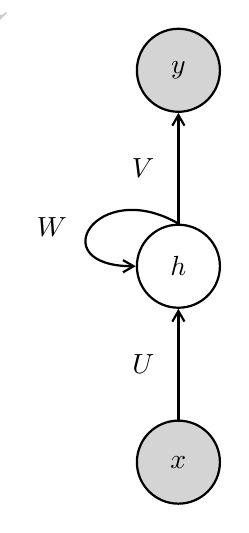
\begin{tikzpicture}
            [align=center]
            % Draw recurrent network
            \node[neuron] (h) {$h$};
            \node[io, below=4em of h] (x) {$x$};
            \node[io, above=4em of h] (y) {$y$};

            \draw[conn] (h) -- node [left=0.5em, midway, align=center] {$V$} (y);
            \draw[conn] (x) -- node [left=0.5em, midway, align=center] {$U$} (h);
            \draw[conn] (h.north) to [out=150, in=180, loop, looseness=4] node[left=0.5em, midway, align=center] {$W$} (h.west);

        \end{tikzpicture}
        \caption{Folded}
        \label{fig:rnn_folded}
    \end{subfigure}
    \begin{subfigure}{.74\linewidth}
        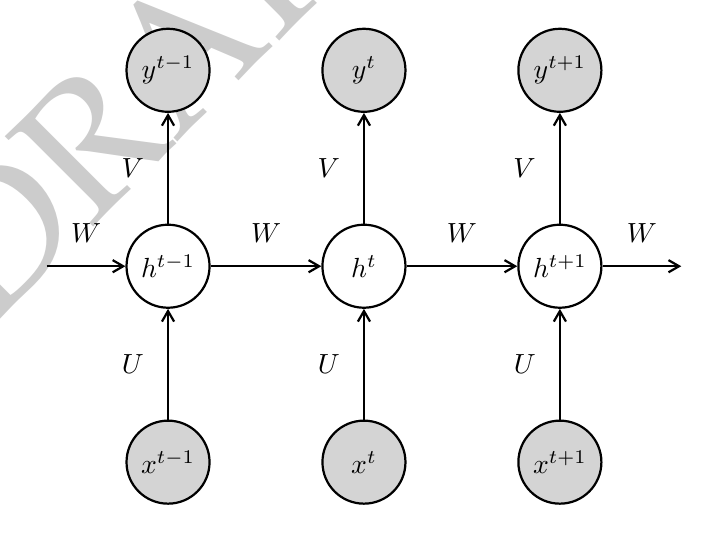
\begin{tikzpicture}
            [align=center]
            % Draw middle unfold
            \node[neuron] (ht) {$h^t$};
            \node[io, below=4em of ht] (xt) {$x^t$};
            \node[io, above=4em of ht] (yt) {$y^t$};

            \draw[conn] (ht) -- node [left=0.5em, midway, align=center] {$V$} (yt);
            \draw[conn] (xt) -- node [left=0.5em, midway, align=center] {$U$} (ht);

            % Draw left unfold
            \node[neuron, left = of ht] (ht-1) {$h^{t-1}$};
            \node[io, below=4em of ht-1] (xt-1) {$x^{t-1}$};
            \node[io, above=4em of ht-1] (yt-1) {$y^{t-1}$};

            \node[left= of ht-1] (nullLeft) {};

            \draw[conn] (ht-1) -- node [left=0.5em, midway, align=center] {$V$} (yt-1);
            \draw[conn] (xt-1) -- node [left=0.5em, midway, align=center] {$U$} (ht-1);

            \draw[conn] (ht-1) -- node [above=0.5em, midway, align=center] {$W$} (ht);
            \draw[conn] (nullLeft) -- node [above=0.5em, midway, align=center] {$W$} (ht-1);
            % Draw right unfold
            \node[neuron, right= of ht] (ht+1) {$h^{t+1}$};
            \node[io, below=4em of ht+1] (xt+1) {$x^{t+1}$};
            \node[io, above=4em of ht+1] (yt+1) {$y^{t+1}$};

            \node[right= of ht+1] (nullRight) {};

            \draw[conn] (ht+1) -- node [left=0.5em, midway, align=center] {$V$} (yt+1);
            \draw[conn] (xt+1) -- node [left=0.5em, midway, align=center] {$U$} (ht+1);

            \draw[conn] (ht) -- node [above=0.5em, midway, align=center] {$W$} (ht+1);
            \draw[conn] (ht+1) -- node [above=0.5em, midway, align=center] {$W$} (nullRight);

        \end{tikzpicture}
        \caption{Unfolded}
        \label{fig:rnn_unfolded}
    \end{subfigure}
    \caption{A typical view of an RNN (left) and an unfolded view of the same network (right). In both sub-figures each node is a layer of network units however, in the second representation these are shown for each timestep. The weighted connections from the input layer to the hidden one is labelled $U$, those from the hidden layer feeding back to itself are $W$, and those from the hidden layer to the output layer are labelled as $V$. Note that these weights are reused at each timestep. Bias has been omitted in this representation. Figure adapted from \textcite{graves_supervised_2012}}
\end{figure}

The LSTM is made of a network of recurrently connected subnetworks known as memory blocks, each with one or more self-connected memory cells and three multiplicative units: the input gate, the output gate, and the forget gate \parencite{hochreiter_long_1997}. The three gates act as analogies for the read, write, reset computer operations and allow the memory cells to store and access information over long periods of time \parencite{graves_supervised_2012}. See Figure \ref{fig:lstm} for an illustration of a LSTM memory block with a single cell.

Aside from being successful at a variety of classification tasks \parencite[e.g.,][]{graves_framewise_2005}, this architecture has been successfully applied to generating new data points \parencite[such as creating sequences of text;][]{graves_generating_2013}. In the context of generating musical performances, experiments with this neural architecture go as far as \textcite{eck_first_2002} however, a more noteworthy implementation is Performance-RNN \parencite{oore_this_2018}; a three layer LSTM network with 512 cells each designed to generate classical compositions whilst maintaining the playing style of expert pianists. Considering its success, this model was re-implemented for the purposes of this paper's experiments (see Chapter \ref{chap:methods}).

\begin{figure}[t]
    \centering
    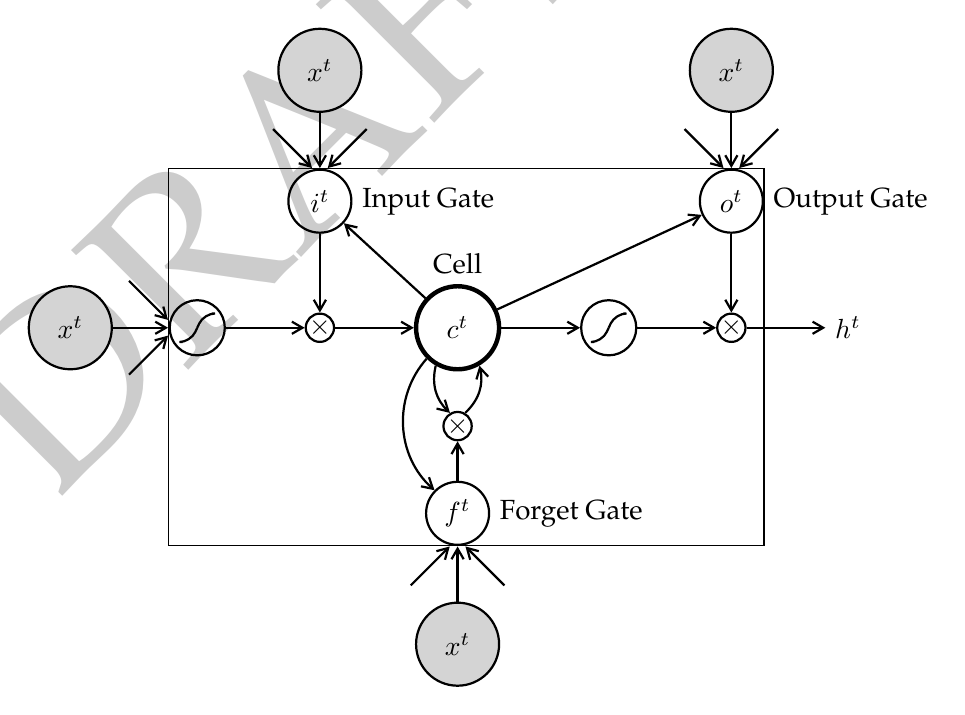
\begin{tikzpicture}
        \node[ct, label={Cell}] (ct) {$c^t$};
        \node[filter, right=of ct] (int1) {};
        \node[prod, right=of int1] (x1) {$\times$}; 
        \node[right=of x1] (ht) {$h^t$};
        \node[prod, left=of ct] (x2) {$\times$}; 
        \node[filter, left=of x2] (int2) {};
        \node[prod, below=5mm of ct] (x3) {$\times$}; 
        \node[ft, below=5mm of x3, label={right:Forget Gate}] (ft) {$f^t$};
        \node[ft, above=of x2, label={right:Input Gate}] (it) {$i^t$};
        \node[ft, above=of x1, label={right:Output Gate}] (ot) {$o^t$};

        \foreach \i/\j in {int2/x2, x2/ct, ct/int1, int1/x1,
                        x1/ht, it/x2, ct/it, ct/ot, ot/x1, ft/x3}
                            \draw[->, conn] (\i)--(\j);

                            \draw[->, conn] (ct) to[bend right=45] (ft);

                            \draw[->, conn] (ct) to[bend right=30] (x3);
                            \draw[->, conn] (x3) to[bend right=30] (ct);

                            \node[fit=(int2) (it) (ot) (ft), draw, inner sep=0pt] (fit) {};

                            \draw[<-, connl] (fit.west|-int2) coordinate (aux)--++(180:7mm) node[left, io]{$x^t$};
                            \draw[<-, connl] ([yshift=1mm]aux)--++(135:7mm);
                            \draw[<-, connl] ([yshift=-1mm]aux)--++(-135:7mm);
                                         
                            \draw[<-, connl] (fit.north-|it) coordinate (aux)--++(90:7mm) node[above, io]{$x^t$};
                            \draw[<-, connl] ([xshift=1mm]aux)--++(45:7mm);
                            \draw[<-, connl] ([xshift=-1mm]aux)--++(135:7mm);
                                          
                            \draw[<-, connl] (fit.north-|ot) coordinate (aux)--++(90:7mm) node[above, io]{$x^t$};
                            \draw[<-, connl] ([xshift=1mm]aux)--++(45:7mm);
                            \draw[<-, connl] ([xshift=-1mm]aux)--++(135:7mm);
                                          
                            \draw[<-, connl] (fit.south-|ft) coordinate (aux)--++(-90:7mm) node[below, io]{$x^t$};
                            \draw[<-, connl] ([xshift=1mm]aux)--++(-45:7mm);
                            \draw[<-, connl] ([xshift=-1mm]aux)--++(-135:7mm);
    \end{tikzpicture}
    \caption{LSTM memory block with one cell. Here the gates are nonlinear summation units that collect activations from the inside and outside of the memory block and control the activation of the cell $c^t$ via multiplications. The input and output gates ($i^t$, $o^t$) multiply the block's input and output activations respectively, while the forget gate ($f^t$) multiplies the previous hidden state. The input and output activation are typically tanh or sigmoid. The only outputs ($h^t$) from the block come from the output gate multiplication. Figure adapted from \textcite{graves_supervised_2012}}
    \label{fig:lstm}
\end{figure}

\section{Generative Adversarial Networks} \label{sec:generative}

Nowadays, the most popular form of generating data is through the use of a Generative Adversarial Network \parencite[GAN;][]{goodfellow_generative_2014}. The training procedure is set up as a game between two networks: a generator and a discriminator. The purpose of the former is to create samples that come from the same distribution as the training data, whereas the latter aims to determine which samples are real or fake \parencite{goodfellow_nips_2016}.

To make the generator's data distribution $p_g$ imitate that of the real data $p_{\text{data}}$, we need to define a prior on input noise variables $p_{z}(z)$ and then represent a mapping to the data space $G(z; \theta_g)$ where $G$ is a differentiable function represented by a network with parameters $\theta_g$. The discriminator is another network with a mapping function $D(x; \theta_d)$ that outputs a single scalar. More concretely, $D(x)$ is the probability that $x$ came from the real data distribution rather than that of the generator \parencite{goodfellow_nips_2016}. We train $D$ to maximize the probability of correctly classifying the training data and samples from $G$ (i.e., as "real" and "fake"), while simultaneously training $G$ to minimize the dissimilarity between the two data distributions, \emph{without actually looking at} $p_{\text{data}}$. In other words, $G$ must minimize $\log (1- D(G(z)))$ \parencite{goodfellow_generative_2014}.

To formalize, both models play a minimax game with a value function $V(G, D)$:
\begin{equation}
    \min_G \max_D V(D, G) = \mathbb{E}_{x ~ p_{\text{data}}} [ \log D(x) ] + \mathbb{E}_{z ~ p_z (z)} [ \log (1-D(G(z))) ]
\end{equation}
where the solution is for $G$ to recover the training data distribution and $D$ to have a classification accuracy of 50\% \parencite{goodfellow_generative_2014}.

Although new, GANs are a significant conceptual and technical innovation \parencite{briot_deep_2017} which can be seen in them revitalizing interest in generative models. As mentioned before, they have been proven successful at image super-resolution \parencite{ledig_photo-realistic_2016}, image-to-image translation \parencite{isola_image--image_2016}, or style-based image generation \parencite{karras_style-based_2018}. Having said these, \textcite{mogren_c-rnn-gan_2016} has shown that GANs do not belong only to the field of Computer Vision by successfully re-purposing this architecture to generate music. The model in question, C-RNN-GAN, features a completely unidirectional LSTM network with two layers, 350 units each as generator and a unidirectional LSTM network with a similar structure as discriminator.

\section{Learning to learn} \label{sec:learn2learn}

The rationale for investing time and energy into meta-learning is that we cannot capture the essence of learning simply by relying on a small number of algorithms, but rather a bunch of context-dependent learning strategies that would enable us to properly capture domain specific information \parencite{schmidhuber_evolutionary_1987}. Given the complexities of each learning strategy, \textcite{schmidhuber_evolutionary_1987} argues that an obvious way to tackle this initiative is to give a system the ability to learn how to learn. A simplistic way to do this would be to train a system on different tasks (e.g, image classification, text classification, etc.). However, this approach entails training on a dataset that is much larger that what current hardware can withstand. Furthermore, this approach would stray away from the idea of building general-purpose A.I. architectures as generalizing over a task would require more data points that what a human would need. To be more concrete, a human is able to generalize a task/object after encountering one (or few) example(s) \parencite{ravi_optimization_2016, chen_closer_2018}. Therefore, besides having to perform on a variety of tasks, a system would also need to excel at that using sparse amounts of data.

Although ideas of meta-learning can go as far as Schmidhuber's thesis in 1987, it seems that training a model using a handful of examples did not get much traction until \textcite{lake_human-level_2015} successfully designed a probabilistic learning framework capable of generalizing and learning a large number of concepts from a single class example (i.e., one-shot learning). For clarity, such a problem is typically defined as a $n$-shot $k$-way problem, where $n$ stands for the number of examples per class, and $k$ is the number of classes to be used in the training process.

Initially, it was thought that ANNs are incompatible with few-shot learning since the iterative nature of gradient-based optimization algorithms do not work well in the context of a set number of updates \parencite{ravi_optimization_2016} - and even more so when there are only a few examples to work with. Having said that, \textcite{rezende_one-shot_2016} were among the first to provide a solution to the one-shot problem in the context of a neural network by implementing Bayesian reasoning into a deep network embedded within hierarchical latent variable models. Since that, numerous efforts were made to develop an algorithm that enables an ANN to perform with strictly limited datasets. Probably the most popular algorithm at the time of writing is the Model-Agnostic Meta-Learning (MAML) algorithm \parencite{finn_model-agnostic_2017}. One of MAML's core mechanics is that the parameters of the model are trained with a small number of gradient steps on with little training data to arrive at a good generalization on that task. However, this procedure requires calculating second-order derivatives which implies a substantial computational penalty - something which the authors did note. Therefore, they developed a first-order variant of MAML (FOMAML) which is able to perform similarly, if only with a small performance hit \parencite{finn_model-agnostic_2017}.

This seemed to be the case until \textcite{nichol_first-order_2018} showed that FOMAML tends to be somewhat unstable. In response to that, they developed Reptile, a first-order meta-learning algorithm that rivals the performance of both MAML and FOMAML \parencite{nichol_first-order_2018}. Just like MAML, it counteracts the shortcomings of gradient-optimization algorithms by learning the model's initial parameters in order to maximize performance on novel tasks, it allows for any type of network to be used, and does not place any restrictions on the type of loss function that can be used \parencite{nichol_first-order_2018}. The difference between the two, however, lies in the way the parameters are updated. 

\IncMargin{1em}
\begin{algorithm}
Initialize $\theta$, the vector of initial parameters

\For{iteration = $1, 2, \dots$}{
    Sample task $\tau$, corresponding to loss $L_{\tau}$ on weight vectors $\tilde \theta$

    Compute $\tilde \theta = U_{\tau}^{k} (\theta)$, denoting $k$ steps of SGD or Adam

    Update $\theta \leftarrow \theta + \epsilon (\tilde{\theta} - \theta)$
}

\caption{Reptile (serial version)}
\label{alg:reptile}
\end{algorithm}
\DecMargin{1em}

In essence, Reptile works (see Algorithm \ref{alg:reptile}) as follows. A model with parameters $\theta$ is initialized, and a meta-loop (or meta-epochs) of $i$ iterations starts. Within it, a task $\tau$ (e.g, image classification, text classification, etc.) is sampled, along with its corresponding loss function $L_{\tau}$ (for clarity, we assume that each type of task uses a different loss function). Then we compute the updated parameters $\tilde \theta$ in an inner-loop with $k$ iterations on task $\tau$ (or in other words, once we sampled our task $\tau$, we train our model $k$ times on it using the $\theta$ as parameters so we can get $\tilde \theta$). Finally, we update our initial parameters $\theta$ using this formula: $\theta \leftarrow \theta + \epsilon (\tilde{\theta} - \theta)$. Then the algorithm continues to the next iteration of the meta-loop carrying over our updated parameters $\theta$.

The explanation above is fairly verbose however, the algorithm itself is fairly simplistic and achieves similar performances to FOMAML \parencite{nichol_first-order_2018}. This forms a compelling reason to use Reptile as the few-shot learning method of choice for this paper.

\chapter{Methods}\label{chap:methods}

To reiterate from Section \ref{sec:thesis_goal}, the purpose of this paper is to establish (1) the extent to which the music generated under a few-shot learning algorithm is comparable to that of a model trained on the entire dataset, and (2) the extent to which the music from such a model is comparable to that of real musical performances. For these purposes, Performance-RNN and C-RNN-GAN were adapted to the Reptile training procedure (Algorithm \ref{alg:reptile}) and evaluated against the (1) songs generated by the baseline proposed in \textcite{larochelle_few-shot_2017} - a single layer LSTM with 256 units - and (2) actual musical performances from the dataset (Section \ref{sec:dataset}). For an in-depth explanation on the steps required to develop a model that is able to generate new data points refer to Section \ref{sec:how_to_gen} and to Section \ref{sec:reptile_train} for details on the training procedure. The evaluation of the models' performances will be based on the number of statistically different bins \parencite[NDB;][]{richardson_gans_2018} and several domain specific measurements adapted from \textcite{mogren_c-rnn-gan_2016}: polyphony, scale consistency, repetitions, tone span. Refer to Section \ref{sec:evaluation} for more details on these metrics.

\section{Dataset} \label{sec:dataset}

The dataset for this research will be similar to that of \parencite{oore_this_2018} namely, the MAESTRO Dataset \parencite{hawthorne_enabling_2018}. It consists of recorded MIDI data collected from each installment of the International Piano-e-Competition. All performances were done by piano experts on a Yamaha Disklavier, instrument which integrates a highly precise MIDI capture and playback system. The claim is that the recorded MIDI events are of sufficient fidelity to allow judges to remotely listen to the contestant's performance (also on a Disklavier).

The dataset contains MIDI recordings from nine years of the International Piano-e-Competition. This amounts to 1,184 piano performances, approximately 430 compositions, 6.18 million notes played, and approximately 172 hours of playback. There is also a recommended train/validation/test split (954, 105, 125 songs respectively) created on the following criteria \parencite{hawthorne_enabling_2018}:

\begin{itemize}
    \item No composition should appear in more than one split
    \item Training set is approx 80\% of the dataset (in time), and the remaining is split equally on between the validation and test sets. Where possible, these proportions are true also within each composer.
    \item Popular compositions are in the training set
    \item The validation and test splits should maintain a variety of compositions
\end{itemize}

Moreover, each performance comes with additional metadata: the name of the composer, the title of the performance, the suggested train, validation, test splits, year of the performance, name of the file, and duration in seconds of the performance. Having said that, the dataset lacks clearly defined classes. The canonical composer could be used as a substitute however, the author strongly believes that there is a better way to categorize music: by genre.

Broadly speaking, Western classical music can be segregated into a number of genres based on the year of the composition and style of the piece. For this we can use the Concise Oxford Dictionary of Music \parencite{kennedy_concise_2007} which indicates to the following classical genres: baroque (1600 - 1750), classical (1750 - 1820), romanticism (1780 - 1910), modernism (1890 - 1930), and impressionism (circa 1890 - 1925). Granted, there are far more genres, but these are the ones that are covered by the dataset. As such, given the definitions of \textcite{kennedy_concise_2007} on said genres and artists, each individual piece from our dataset was manually assigned a genre. Concretely, the style of music was firstly determined by the period in which the composer has lived (in baroque, classical, etc.) or - if the time period of the genres would overlap (the case of modernism and impressionism) - the composer's primary style of music would be chosen according to the definition given by \textcite{kennedy_concise_2007}. Said labelling can be found in Appendix \ref{appendix:labelling}.

\section{Data Processing} \label{sec:data_proc}

\begin{figure}[t]
    \centering
    \begin{verbatim}
<note_on note=69 velocity=73 time=33>
<note_on note=71 velocity=78 time=15>
<control_change control=64 value=83 time=27>
<note_off note=69 velocity=0 time=6>
<note_off note=71 velocity=0 time=3>
    \end{verbatim}
    \caption{Example of MIDI messages in the dataset, as printed by the Python library Mido \parencite{bjorndalen_mido_2018}. At 33 ticks since the last event, the player pressed an A4 (note 69), followed by a B4 (note 71), 15 ticks later. Next, the pedal (Control Change message with a value of 64) is pressed 27 ticks later, and the keys are released 6 and 3 tick later.}
    \label{fig:midi_examples}
\end{figure}

The dataset consists of MIDI files which would require some processing in order to be ready for a LSTM network. Here, the approach of \textcite{oore_this_2018} was adopted where MIDI midi messages are transformed into a sequence of one-hot encoded events. More specifically, MIDI excerpts are represented as a sequence of events from a vocabulary of 416 different events - similar to \textcite{oore_this_2018}, but with one extra events in the vocabulary:
\begin{itemize}
    \item 128 Note-On events: starts a new note (one for each of the 128 MIDI pitches)
    \item 128 Note-Off events: releases a note (one for each of the 128 MIDI pitches)
    \item 126 Time-Shift events: moves the time step forward somewhere between 0 ms and 1 second, in increments of 8 ms (\textcite{oore_this_2018} ignored the 0ms forward step)
    \item 32 Velocity events: changes the velocity for each subsequent note, until the next velocity event
    \item 2 Pedal events: triggers or releases the pedal
\end{itemize}

A glance over the MIDI documentation \parencite{midi_association_official_2019} shows how complex and granular the standard is. Luckily however, we do not need to implement all of the messages into our model in order to make it work. We only need three: \texttt{note\_on}, \texttt{note\_off}, and \texttt{pedal\_on/off}. Figure \ref{fig:midi_examples} show an example of how the midi messages look like. It should be noted that in this figure, the time is represented in ticks, MIDI's smallest unit of time, who's value is usually a third of a beat \parencite{midi_association_official_2019}.

As it can be seen in Figure \ref{fig:midi_examples}, each message contains multiple pieces of information such as the message type, the note/value of the message, the delta time (time elapsed since last message and the current message, measured in ticks), and velocity (if applicable). To one-hot encode this stream of messages, it is necessary to separate it so it contains only one type of information per input. Thus, the sequence can be further broken down such that the first message that the system encounters is the delta time, followed by the velocity, and the note/pedal event (and their respective values). An example of how the MIDI sequences are broken down into singular pieces of information can be found in Figure \ref{fig:representation_midi}.

\begin{figure}[t]
    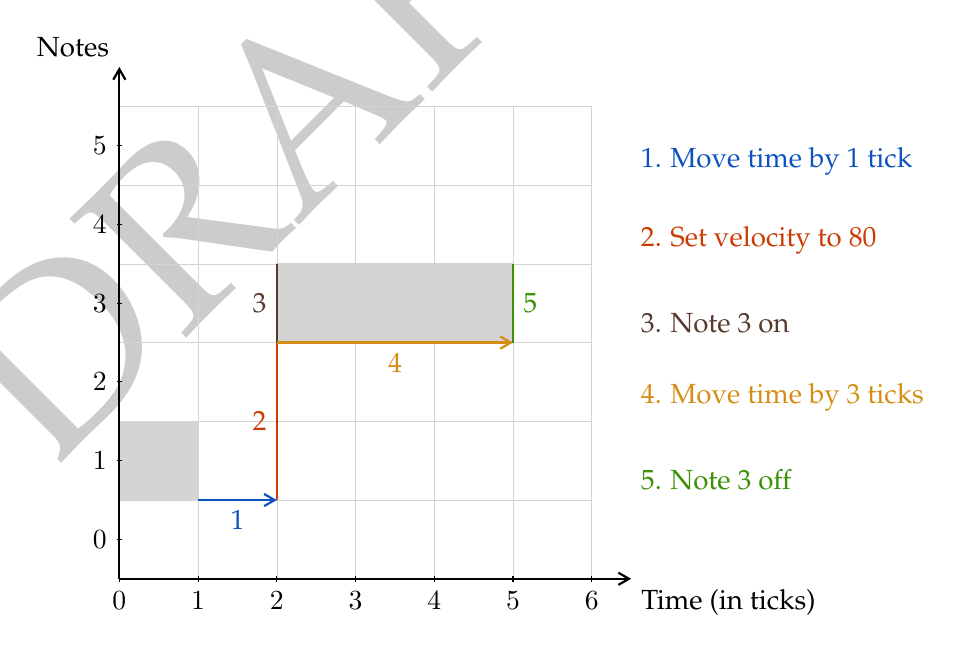
\begin{tikzpicture}
        \draw[step=1cm,base01,very thin] (0,0) grid (6,6);
        \filldraw[fill=base01, draw=base01] (0,1) rectangle (1,2);
        \filldraw[fill=base01, draw=base01] (2, 3) rectangle (5, 4);
        \draw (6.5, 5) node[anchor=south west, color=base09] {1. Move time by 1 tick};
        \draw (6.5, 4) node[anchor=south west, color=base0A] {2. Set velocity to 80};
        \draw (6.5, 3) node[anchor=south west, color=base0B] {3. Note 3 on};
        \draw (6.5, 2) node[anchor=south west, color=base0C] {4. Move time by 3 ticks};
        \draw (6.5, 1) node[anchor=south west, color=base0D] {5. Note 3 off};

        \draw[ -{Straight Barb[angle=60:2pt 3]}, color=base09, thick] (1, 1) -- (2, 1) node[anchor=north, midway] {1};
        \draw[color=base0A, thick] (2, 1) -- (2, 3) node[anchor=east, midway] {2};
        \draw[color=base0B, thick] (2, 3) -> (2, 4) node[anchor=east, midway] {3};
        \draw[ -{Straight Barb[angle=60:2pt 3]}, color=base0C, thick] (2, 3) -- (5, 3) node[anchor=north, midway] {4};
        \draw[color=base0D, thick] (5, 3) -- (5, 4) node[anchor=west, midway] {5};

        \draw[thick,-{Straight Barb[angle=60:2pt 3]}] (0,0) -- (6.5,0) node[anchor=north west] {Time (in ticks)};
        \draw[thick,-{Straight Barb[angle=60:2pt 3]}] (0,0) -- (0,6.5) node[anchor=south east] {Notes};
        \foreach \x in {0,1,2,3,4,5,6}
           \draw (\x cm,1pt) -- (\x cm,-1pt) node[anchor=north] {$\x$};
        \foreach \y in {0,1,2,3,4,5}
            \draw (1pt,\y.5 cm) -- (-1pt,\y.5 cm) node[anchor=east] {$\y$};
    \end{tikzpicture}
    \caption{Example of how the data is represented. The progression illustrates how a piano roll of MIDI data is converted into a sequence of commands (right hand side) that belong to our events vocabulary. Figure adapted from \textcite{oore_this_2018}.} 
    \label{fig:representation_midi}
\end{figure}

Having said these, it should be mentioned that the one-hot representation of MIDI messages has undergone some fine quantization, again, in a similar fashion to \textcite{oore_this_2018}. The delta times have been modified to correspond to a change of multiples of 8 ms (i.e., 0 ms, 8 ms, 16 ms, etc.) and the velocities have been partitioned into 32 steps as opposed to MIDI's 128. With regards to the time movements, \textcite{friberg_overview_2006} note that a noticeable difference in temporally displacing a single tone in a sequence takes place from 10 ms and above. Thus, since our movements are quantized in steps of 8 ms, there should be no discernible difference for the human hearing. When it comes to the note velocities, it should be pointed to the reader that classical music features eight levels of common dynamic marking (from $ppp$ to $fff$) which is why \textcite{oore_this_2018} note that 32 steps are more than enough.

\section{How to make music} \label{sec:how_to_gen}

Knowing what we know about RNNs and LSTMs from Section \ref{sec:rnn}, one can devise a method where the network can generate a sequence of events. All that is needed is to present the system with an event to kickstart the generative process. Namely, an input $x^t$ is fed to the network in order to output the next likely event $x^{t+1}$, which in turn is fed back to generate $x^{t+2}$. This process is repeated until we have a sequence of events of a desired length.

An alternative to this would be to define a noise vector $z^t$ of an arbitrary size (e.g., 100), and a random input $x^t$ selected from our events vocabulary. The noise vector is passed through a linear layer that output a tensor that would serve as the network's hidden state $h^{t}$ at time $t$. It is then that $x^t$ and $h^{t}$ are fed into the LSTM layer to generate $x^{t+1}$ and $h^{t+1}$. The reason for pre-defining the hidden state for the first input is to increase the number of possible outcomes coming from the network.

To be more precise, if we were to present the network with only $x^t$ then the network would mark the input sequence as the beginning of the song. With that information, it is possible that the network would affix itself to following a specific pattern. For instance, if the first input would be a C\#, the network could learn to always output E as the next note. Using a random hidden state is a measure that was placed to ensure some diversity in the process of generating samples (granted, it should be admitted the possibility of this scenario being unlikely, and that the regular method described at the beginning of this section would still work just as good).

Having said this, diversity is not the only reason for including a noise vector $z$ into the training process. The reader might recall that this is part of the generation process in the framework of a GAN respectively, how the generator $G$ would create samples. As such, all three models implemented in this paper feature the architecture of a GAN generator.

Moreover, in terms of generating the next event, \textcite{oore_this_2018} have defined a parameter $\lambda$ called temperature \parencite{google_magenta_performance_2017}. It is a value which uses the model's predicted events distribution to control the randomness of the output samples. In other words, let $\phi$ be the output of a LSTM network (for clarity, we ignore the hidden state $h$). Then, the next sequence $x^{t+1}$ is defined as 
\begin{equation}
    x^{t+1} = X(\omega)
\end{equation}
where
\begin{equation}
    X = \text{softmax}(\phi / \lambda).
\end{equation}
$X$ is the predicted event distribution of the network's output divided by our temperature $\lambda$. Thus, $x^{t+1}$ is actually a random sample from our defined categorical distribution $X$. In this paper we train our models with a temperature of 1.0, and generate samples with temperatures ranging from 0.8 to 1.2, with an increment of 0.1.

\section{Training procedure} \label{sec:reptile_train}

With the generative process outlined in the previous section, training the generative networks presented in this papers is somewhat straightforward. A batch of songs is sampled from the training set, the model generates as many songs as there are in the batch, and then compute the loss between the network's output and the real samples. This statement is essentially true for the baseline and Performance-RNN (in spite of the Reptile training procedure, inner-loop training is similar to the standard procedure). In contrast, the GAN model requires training two models simultaneously, where the generator's loss function is based on whether the discriminator is fooled by the fake samples (i.e., classifies them as real), and the discriminator's loss is based on whether it can distinguish between real and fake samples (it should be mentioned that both components of the GAN would use binary cross-entropy as their loss function; in contrast the baseline and Performance-RNN are based on cross entropy). However, there are still several items that we haven't touched upon.

Firstly, all three networks have been trained with teacher forcing, a procedure in which during training the model receives the ground truth $y^t$ as input at time $t+1$. Adopting this measure allows the model to create hidden-to-hidden connections and capture the necessary information from the history of input sequences \parencite{goodfellow_deep_2016}.

Secondly, \textcite{goodfellow_generative_2014} mention a couple issues that can arise when training a GAN. One is synchronizing the generator with the discriminator (it's possible that one of the models gets too strong, leaving the other unable to catch up), and the generator collapsing too many values of $z$ to the same value of $x$ (which would ultimately hurt the generator's diversity; this issue is known in the literature as mode collapse).

A solution to the issue of synchronicity would be to freeze the training of one of the models when the loss is below a predefined threshold \parencite{mogren_c-rnn-gan_2016}. In this paper, we stop training one of the models if its training loss is less than half the loss of the other's.

To combat mode collapse, \textcite{salimans_improved_2016} propose a technique called feature matching, where we change the objective of the generator to generate real data that matches the statistics of the real data. Since in the setting of a GAN showing the real data would be considered "cheating", we use the features of an intermediate layer of the discriminator. Specifically, we train the generator to match the expected value of those features \parencite{salimans_improved_2016}. Denoting $f(x)$ as the activations on an intermediate layer in the discriminator, the new objective for the generator becomes
\begin{equation}
    \|\mathbb{E}_{x~p_{data}} f(x) - \mathbb{E}_{z~p_z (z)} f(G(z))\|_2^2
\end{equation}
which is commonly known as the squared error. However, to make the re-implementation of C-RNN-GAN true to the original, Mean Square Error (MSE) was used as the loss function when using feature matching.

It should be noted that now, the loss functions of both the generator and discriminator differ in scale, meaning that we can no longer compare them to freeze training of either models: the generator uses MSE, whereas the discriminator use binary cross-entropy. A workaround to this is to calculate the both losses, but use MSE for backpropagation and optimization, whilst binary cross-entropy is used to compare our models.

Moving forward, there is an aspect pertaining to the Reptile training framework which needs to be addressed: the training data. Normally, Reptile assumes that the training takes place in the $n$-shot $k$-way setting, meaning that our model is trained with $k$ classes and $n$ samples per class. Given that we have 954 samples in the training set, we adopted the same training procedure as \textcite{nichol_first-order_2018} and \textcite{clouatre_figr_2019}. Respectively, at each meta-loop we sample from our split $n$ examples for each $k$ class. For this paper, our $n=1$ and $k=5$ corresponding to a 5-way 1-shot experiment.

Another aspect that needs addressing is the number of epochs. All models were trained for 250 epochs each however, when looking at the way training is handled in Reptile (see Algorithm \ref{alg:reptile}), this statement is inconclusive. Because the algorithm presents us with a meta-loop and an inner-loop, epochs is defined in this setting as the number of times parameters $\theta$ have been updated. Thus, the number of steps we have taken to compute $\tilde \theta$ is ignored. If this claim causes any skepticism about whether the models trained under Reptile would outperform simply because they "are trained much more", the reader should be reminded by the fact that the baseline is presented with 954 songs per epoch, whereas these models are trained with five.

With these in mind, it should be mentioned that neither of the three models was presented with a full song during training, but rather with each song split into fixed-size chunks. This decision was made to better accommodate the memory limits of the hardware (an Nvidia T4 GPU). A full explanation of the limitations is found in Appendix \ref{appendix:memory}. It suffices to say that our dataset won't fit in memory. As such, each song was split into chunks of 200 events (i.e., window size of 200), starting from the beginning and moving towards the end of the song at a rate of 50 events per chunk (i.e, stride size of 50). Thus, a song of, say, 800 events would be transformed into 13 chunks, which leads us to the topic of batch size.

At training, the Reptile models were presented with batches of 64 chunks, whereas the baseline was presented with batches of 2048 chunks. The rationale for the latter is that training of the baseline under a regimen of 64 batches would take approximately 250 hours until completion.

Finally, another aspect that needs addressing is the learning rate. The baseline and Reptile inner-loop training was conducted with an $\alpha = 0.001$, value borrowed from \textcite{oore_this_2018}. Since Reptile also dictates a learning rate for the meta-loop, this value was set to $\beta = 0.01$. The reason for choosing this value comes from the Reptile experiments done by \textcite{nichol_first-order_2018}, where the meta-loop learning rate tends to be ten times higher than the inner rate. 

A summary of the parameters used in the training procedures is found in Table \ref{tab:params}.

\begin{table}[ht]
    \centering
    \begin{tabular}{l|c|c|c}
                    &\bf Baseline   &\bf Performance RNN&\bf C-RNN-GAN  \\ \hline
    Num. Layers     &   1           &   3               &   2           \\
    Num. Units      &   256         &   512             &   350         \\
    Dropout Rate    &   0.0         &   0.3             &   0.3         \\
    Learning Rate   &   0.001       &   0.001           &   0.001       \\
    Meta Rate       &   N/A         &   0.01            &   0.01        \\
    Batch Size      &   2048        &   64              &   64          \\
    Meta Epochs     &   250         &   250             &   250         \\
    Inner Epochs    &   N/A         &   3               &   3           \\
    Has bias vector &   No          &   Yes             &   Yes         \\
    Gradient Clipped&   No          &   Yes             &   Yes         \\
    \end{tabular}
    \caption{Summary of parameters used to construct and train the three models featured in this paper}
    \label{tab:params}
\end{table}

\section{Evaluation} \label{sec:evaluation}

Generally, DL models work by the principle of likelihood maximization, which simply says to choose the parameters that maximize the probability that the model assigns to the training data \parencite{goodfellow_nips_2016}. Formally, this means selecting the parameters that maximize $\prod_{i=1}^N p_{\text{model}}(\bm{x}^{(i)}; \bm{\theta})$:

\begin{equation}
    \bm{\theta^*} = \arg \max \prod_{i=1}^N p_{\text{model}}(\bm{x}^{(i)}; \bm{\theta}) \label{eq:og_mle}.
\end{equation}

However, calculating the product over many probabilities is prone to numerical problems such as underflow \parencite{goodfellow_nips_2016}. This is alleviated by calculating $\bm{\theta^*}$ in $\log$ space where the product is transformed into a sum:

\begin{equation}
    \bm{\theta^*} = \arg \max \sum_{i=1}^N \log p_{\text{model}}(\bm{x}^{(i)}; \bm{\theta}) \label{eg:log_mle}.
\end{equation}

That being said, calculating maximum likelihood can be thought of minimizing the Kullback-Leibler (KL) divergence: minimizing the dissimilarity between the data generating distribution $p_{\text{data}}$ and the model $p_{\text{model}}$. Thus, $\bm{\theta^*} = \argmin_{\bm{\theta}} D_{KL}(p_{\text{data}}(\bm{x}) \| p_{\text{model}} (\bm{x}; \bm{\theta}))$. The KL divergence is given by:

\begin{equation}
    DL_{KL} = \mathbb{E}_{\mathbf{x} \sim p_{\text{data}}} [\log p_{\text{data}} (\bm{x}) - \log p_{\text{model}} (\bm{x})] \label{eq:kl_div}.
\end{equation}

Having all these in mind, $\log p_{\text{data}}$ is a result of the data-generating process, and not the model. Therefore, a final simplification is applied where the maximum likelihood estimate would be calculated as:

\begin{equation}
    \bm{\theta^*} = - \mathbb{E}_{\mathbf{x} \sim p_{\text{data}}} [\log p_{\text{model}} (\bm{x})] \label{eq:nll}.
\end{equation}

Note that Eq. \ref{eg:log_mle} is the same as Eq. \ref{eq:nll}. The reason why this is brought up, is because negative log-likelihood (NLL; Eq. \ref{eq:nll}) is used both as a loss function and as an evaluation metric \parencite[also for generative models;][]{yu_seqgan_2016, borji_pros_2018}.

However, as \textcite{borji_pros_2018} notes, NLL is uninformative about the quality of the samples generated and it does not allow to answer whether the generative network is simply memorizing training examples. As such, this study will rely on other evaluation metrics when assessing generative models: the number of statistically different bins \parencite[NDB;][]{richardson_gans_2018}, polyphony, scale consistency, repetitions, and tone span \parencite{mogren_c-rnn-gan_2016}.

NDB is an evaluation metric specifically designed for generative models to measure the diversity of the generated samples. It follows the intuition that given two samples from the same distribution, the number of samples that fall into a bin (read as: class or cluster) should be the same \parencite{richardson_gans_2018}. Let $I_B(\mathbf{x})$ be the indicator function for bin $B$. Then $I_B(\mathbf{x}) = 1$ if the sample falls into $B$, and zero otherwise. Let also $\{\mathbf{x}_i^p\}$ define $N_p$ samples from a $p$ distribution (e.g., test set samples) and $\{\mathbf{x}_i^q\}$ be the $N_q$ samples from a $q$ distribution (e.g., generated samples). If $p = q$ then the followings is also true:

\begin{equation}
    \frac{1}{N_p} \sum_i I_B(\mathbf{x}_i^p) \approx \frac{1}{N_q} \sum_i I_B(\mathbf{x}_i^q)
\end{equation}

The pooled sample proportion $P_B$ is the proportion of samples (from the joined sets) that fall into $B$. The standard error for bin $B$ is given by:

\begin{equation}
    SE_B = \sqrt{P_B (1 - P_B)[1 / N_p + 1 / N_q]}
\end{equation}

The test statistic is a $z$-score $z = \frac{P_B^p - P_B^q}{SE_B}$ where $P_B^p$ and $P_B^q$ are the proportions of each sample that fall into $B$. If $z$ is smaller than a threshold (a significance level such as $\alpha = 0.05$), then the samples within that bin are statistically different. This whole process is repeated for each bin, and the number of statistically different bins is reported. The selection of bins is done through a $K$-means clustering performed on the $\mathbf{x}^p$ samples. Each of the generated samples $\mathbf{x}^q$ is by assigned to the nearest $L_2$ $K$ centroid \parencite{richardson_gans_2018}.

The more domain-specific evaluation measures are adapted from \textcite{mogren_c-rnn-gan_2016}. Polyphony measures how often a minimum of two tones are played simultaneously (when the start time is the same). It should be noted that this is a restrictive metric: it can give a low score to music where the two notes start at different times. Scale consistency is the fraction of notes that are part of a standard scale (e.g., major, minor, lydian, etc.; see Appendix \ref{appendix:scales} for a complete list with examples), and reporting the results for the best matching scale. Repetitions counts consecutive subsequences of notes, and tone span is the difference between the lowest note and highest note \parencite[counted in semi-tones;][]{mogren_c-rnn-gan_2016}.

The choice of NDB comes from the fact that it is good at detecting overfitting \parencite{borji_pros_2018}, whereas the domain-specific metrics should favor models that generate high fidelity samples. In addition, these evaluation metrics have the benefit of being model-agnostic; they do not require a specific type of generative model.

\section{Utilities}

All of the experiments have been conducted in the programming language Python version 3.7.3 \parencite{rossum_python_2019} on a Nvidia T4 GPU as provided by Google Colaboratory \parencite{google_colaboratory_2019}. The models have been built entirely with PyTorch version 1.0.1 \parencite{paszke_automatic_2017}, while the dataset has been processed with a combination of libraries: mido version 1.2.9 \parencite{bjorndalen_mido_2018} for MIDI processing, numpy version 1.16.3 \parencite{walt_numpy_2011} and pandas version 0.23.4 \parencite{mckinney_data_2010} for processing arrays and data frames. Finally, scikit-learn version 0.20 \parencite{pedregosa_scikit-learn_2011} was used for its implementation of $K$-means clustering. The PyTorch reimplementation of Performance-RNN made by \textcite{lee_event-based_2019} was used as an example for developing all three models featured in this paper.

\chapter{Results}\label{chap:results}

To establish the degree to which the music of a Reptile-based model is comparable to (1) a model trained on whole dataset and (2) songs from the dataset, a total of three models have been trained (see Table \ref{tab:params} for a list of training parameters). Training of the baseline finished after 27 hours, 9 hours for the Reptile adaptation of Performance-RNN, and 19 hours for the Reptile adaptation of C-RNN-GAN.

Afterwards, the three have been tasked to generate 125 songs of variable lengths - between 90\% and 110\% of the median length (34,222) of songs in the training set - with five different temperature settings ranging from 0.8 to 1.2. The generating process took approximately 1 hour per model per temperature. The resulting samples were then evaluated against the samples in the test set using the metrics described in Section \ref{sec:evaluation}: polyphony, repetitions, tone span, scale consistency, and number of statistically different bins ($N_{bins} = 20$; arbitrary choice).

The results in Table \ref{tab:results} underline several things about the trained models, the most important one being that all three lack the concept of motif (the presence of a dominant/recurring theme within a piece). The clear giveaway sign is the substantial lack of repetition in the generated samples. This is enforced by the larger levels of polyphony in the three models when compared to the test set. In addition, all models seems to be unrestrained with respect to using the whole gamut of notes they have available, but considering that a piano keyboard has 88 keys and the MIDI standard allows for 128 values (notes), it seems that our models might be heading into the right direction. When it comes to playing in a scale, all models show are equal across the board, with extremely minor variations. Having said these, the domain-specific evaluation metrics indicate that the models are fairly close to eachother but that should not change the fact that there is still room for improvement when compared to the real samples.

Having said that, the landscape changes a bit when looking at NDB, our other evaluation metric. With seven to ten bins statistically different (out of 20), our models seem to display a great deal of disparity form the test samples, even though they somewhat agree between themselves - in other words, they don't seem to be very different from each other.

With these result we have gathered enough information to answer our research questions, where we could claim that our C-RNN-GAN implementation produces some of the most best results (as it scores best on 3/4 domain-specific metrics). However, a deep-dive into the performance at training time paints a whole different picture.

\begin{landscape}
\begin{table}[t]
    \centering
\begin{tabular}{l|l|l|l|l|l|l}
    Model             & Temperature & Polyphony       & Repetitions       & Tone Span        & Scale Consistency & NDB     \\ \hline
\textit{Test Set} & N/A         & \textit{0.4915} & \textit{814.3280} & \textit{66.9440} & \textit{0.6827}   & N/A     \\
Baseline          & 0.8         & 0.5707          & \textbf{\color{base0D}388.0160}    & 78.4480          & 0.6770            & 11      \\
Baseline          & 0.9         & 0.6054          & 373.0560          & 81.3120          & 0.6747            & 10      \\
Baseline          & 1.0         & 0.6112          & 347.3600          & 83.0560          & 0.6728            & 10      \\
Baseline          & 1.1         & 0.6292          & 334.4160          & 84.4400          & 0.6722            & \textbf{\color{base0D}7} \\
Baseline          & 1.2         & 0.6060          & 316.8160          & 85.0480          & 0.6726            & 9       \\
Performance-RNN   & 0.8         & 0.5684          & 377.8240          & 78.8400          & 0.6760            & 9       \\
Performance-RNN   & 0.9         & 0.5852          & 364.9680          & 81.4880          & 0.6757            & 8       \\
Performance-RNN   & 1.0         & 0.6219          & 354.0800          & 83.2400          & 0.6730            & 9       \\
Performance-RNN   & 1.1         & 0.6342          & 343.2240          & 84.4640          & 0.6721            & 9       \\
Performance-RNN   & 1.2         & 0.6061          & 312.2480          & 85.2400          & 0.6723            & 10      \\
C-RNN-GAN         & 0.8         & \textbf{\color{base0D}0.5505}    & 369.5760          & \textbf{\color{base0D}77.7920}    & \textbf{\color{base0D}0.6776}      & 9       \\
C-RNN-GAN         & 0.9         & 0.5940          & 370.5040          & 81.4320          & 0.6749            & 9       \\
C-RNN-GAN         & 1.0         & 0.6060          & 348.3520          & 83.2640          & 0.6733            & 8       \\
C-RNN-GAN         & 1.1         & 0.6343          & 340.4160          & 84.6800          & 0.6730            & 11      \\
C-RNN-GAN         & 1.2         & 0.6057          & 313.6080          & 85.0080          & 0.6726            & 10     
\end{tabular}
\caption{Results of the evaluation process of the generated sample. For comparison, relevant statistics of the test samples have been included. The values which are closest to the test sample are in bold and highlighted in green.}
\label{tab:results}
\end{table}
\end{landscape}

\begin{figure}[ht]
    \newlength\figureheight
    \newlength\figurewidth
    \setlength\figureheight{6cm}
    \setlength\figurewidth{6cm}

    \begin{subfigure}{0.5\linewidth}
        \centering
        % This file was created by matplotlib2tikz v0.7.4.
\begin{tikzpicture}

\definecolor{color0}{rgb}{0.12156862745098,0.466666666666667,0.705882352941177}

\begin{axis}[
height=\figureheight,
tick align=outside,
tick pos=left,
title={Loss of baseline model},
width=\figurewidth,
x grid style={white!69.01960784313725!black},
xlabel={Epochs},
xmin=-12.45, xmax=261.45,
xtick style={color=black},
y grid style={white!69.01960784313725!black},
ylabel={Cross-Entropy Loss},
ymin=1.47697713612937, ymax=2.48596777208149,
ytick style={color=black},
ytick={1.4,1.6,1.8,2,2.2,2.4,2.6},
yticklabels={1.4,1.6,1.8,2.0,2.2,2.4,2.6}
]
\addplot [semithick, color0]
table {%
0 2.31965438276529
1 1.90748266159342
2 1.72841882046599
3 1.67083090830308
4 1.64079277733198
5 1.62209568516566
6 1.60910639424737
7 1.5997820095374
8 1.59237445317782
9 1.58587309202323
10 1.58077085362031
11 1.57609616678495
12 1.57282883845843
13 1.56863718135999
14 1.56556297437503
15 1.56317344852365
16 1.55987350614025
17 1.55756959376427
18 1.55523015759312
19 1.55335308324832
20 1.55140009808999
21 1.54957942865216
22 1.54790025634261
23 1.54645098373294
24 1.54524706733915
25 1.54377564329367
26 1.54236130616986
27 1.54106360587936
28 1.53994983577958
29 1.53875074105767
30 1.53776132143461
31 1.53671275480435
32 1.53583626420452
33 1.5348287075758
34 1.53386477409647
35 1.53319302115303
36 1.53275530355481
37 1.53140236494633
38 1.53077502262134
39 1.53022509412124
40 1.52926831319928
41 1.52871815831615
42 1.52795080439403
43 1.52735466223497
44 1.52670784896383
45 1.52613721959866
46 1.52572912063736
47 1.52515069252023
48 1.52459851767008
49 1.52399442058343
50 1.52352995110246
51 1.52311842286816
52 1.52284034685447
53 2.08201283932878
54 2.27280597847242
55 2.24923078257304
56 2.21815349620122
57 2.18346624019054
58 2.15153996990277
59 2.13405245198653
60 2.10608833627059
61 2.08154360892681
62 2.04944787289088
63 2.02706386320866
64 1.99448439908715
65 1.97335221045292
66 1.94045305538636
67 1.9459823069091
68 1.90484330545251
69 1.89872883202938
70 1.90172866101448
71 1.86862718428557
72 1.87432576744602
73 1.85516490729956
74 2.06464964839128
75 2.2362951200742
76 2.19115445361688
77 2.16254542309504
78 2.14401389199954
79 2.12358162036309
80 2.12139381239047
81 2.11333125543136
82 2.10221227373068
83 2.08019041441954
84 2.07399045733305
85 2.08526272212084
86 2.06361692456099
87 2.1066840044581
88 2.08001064738402
89 2.06968119167365
90 2.06308901825776
91 2.13688082649158
92 2.20657321524162
93 2.17250963472403
94 2.14519920257422
95 2.13019714962978
96 2.12253155501989
97 2.12301234843639
98 2.12299783986348
99 2.10721529389803
100 2.13457264292699
101 2.15845726086543
102 2.13793027229034
103 2.14647801965475
104 2.35762134996744
105 2.21484040125058
106 2.18407973417869
107 2.16319174663379
108 2.21750669295971
109 2.15901270738015
110 2.13083790242672
111 2.12034715540134
112 2.13939486443996
113 2.12796616439636
114 2.12732346069354
115 2.24932661194068
116 2.19498278945684
117 2.17331211383526
118 2.14671143258993
119 2.13745845510409
120 2.1322966040327
121 2.21411656588316
122 2.16022506184303
123 2.16612499149946
124 2.14810264339814
125 2.12254721442094
126 2.1210160702467
127 2.11385897031197
128 2.20548087530411
129 2.14076695361963
130 2.12274016267978
131 2.12410216377332
132 2.113054559781
133 2.10617285794937
134 2.11814605616606
135 2.27090751494353
136 2.18957467434498
137 2.1702246889472
138 2.16045612899157
139 2.15590079128742
140 2.22599504314936
141 2.27073655334803
142 2.25600921821136
143 2.25970753912742
144 2.24433516710997
145 2.23234681785107
146 2.22046057994549
147 2.25348691986157
148 2.21585680487064
149 2.21258900142633
150 2.21089209157687
151 2.35385793562119
152 2.26616596086667
153 2.25019804732158
154 2.23846086458518
155 2.27780126780272
156 2.26524928957224
157 2.26815688667389
158 2.26237659041698
159 2.27547979010985
160 2.2547106267168
161 2.2550160535253
162 2.25338476323164
163 2.26921237374728
164 2.31265224688328
165 2.30417190606777
166 2.28442023579891
167 2.27474538523417
168 2.30594346901545
169 2.27834024738807
170 2.2796130713362
171 2.2710016140571
172 2.26808913969077
173 2.26787325395988
174 2.26966017943162
175 2.26610422650209
176 2.24840770088709
177 2.24603314468494
178 2.26086849203477
179 2.24224413300936
180 2.24689646752981
181 2.25781329893149
182 2.24145600944757
183 2.23985256369297
184 2.24224304063962
185 2.2397282318427
186 2.27101741731167
187 2.28163093213852
188 2.2605166601447
189 2.25914300118501
190 2.29632226320413
191 2.27091871603177
192 2.26568376387541
193 2.30668304860592
194 2.28448483118644
195 2.27650254678268
196 2.28757259306999
197 2.28814736008644
198 2.27264380283081
199 2.27234969230799
200 2.31270828327307
201 2.30331242772249
202 2.28742927427475
203 2.28367479718648
204 2.28171212283465
205 2.2805547198424
206 2.30831917375326
207 2.29422347362225
208 2.2900607746381
209 2.29671977059199
210 2.30210904719738
211 2.28959410351056
212 2.28640178361764
213 2.32949189612499
214 2.31450604418149
215 2.29917719960213
216 2.29525766063195
217 2.29324600616327
218 2.29195545671078
219 2.29105440584513
220 2.29033106909348
221 2.28976489718144
222 2.28937533956308
223 2.28897407479011
224 2.28860314419636
225 2.28841160925535
226 2.28810866979452
227 2.28789422145257
228 2.2877425511296
229 2.28752556042029
230 2.4401045613564
231 2.34265867047585
232 2.30958333898049
233 2.30295432129732
234 2.29883761188159
235 2.29590778625928
236 2.29377478418442
237 2.29220035557563
238 2.3384166428676
239 2.3187903160086
240 2.30330108679258
241 2.30075608480435
242 2.29928048126973
243 2.29838281010206
244 2.29785848065065
245 2.29729451812231
246 2.29696175284111
247 2.29664474439162
248 2.30344734914028
249 2.39640578226401
};
\end{axis}

\end{tikzpicture}
        \caption{Baseline loss at training time}
        \label{fig:loss_baseline}
    \end{subfigure}
    \begin{subfigure}{0.5\linewidth}
        \centering
        % This file was created by matplotlib2tikz v0.7.4.
\begin{tikzpicture}

\definecolor{color0}{rgb}{0.12156862745098,0.466666666666667,0.705882352941177}

\begin{axis}[
height=\figureheight,
tick align=outside,
tick pos=left,
title={Loss of Reptile Performance RNN},
width=\figurewidth,
x grid style={white!69.01960784313725!black},
xlabel={Epochs},
xmin=-12.45, xmax=261.45,
xtick style={color=black},
y grid style={white!69.01960784313725!black},
ylabel={Cross-Entropy Loss},
ymin=1.63425633828883, ymax=6.595980106625,
ytick style={color=black}
]
\addplot [semithick, color0]
table {%
0 6.00865532277705
1 4.00652372620323
2 6.37044720806426
3 4.77592716286907
4 4.02876598458541
5 3.59917874395111
6 3.32351125691475
7 2.91125593398445
8 3.20355144414035
9 2.84702679199901
10 2.83502671935342
11 2.97503527998924
12 2.7870355270527
13 2.62073397636414
14 2.73128600915273
15 2.73885617834149
16 2.89925470278245
17 2.74824702739716
18 2.34790902990636
19 2.5542181965995
20 2.54471276896869
21 2.45493820795776
22 2.49410646431374
23 2.6058038936721
24 2.59644664435023
25 2.56218505109477
26 2.38809664850313
27 2.43033917582765
28 2.47963244156819
29 2.50702665646871
30 2.26822980790356
31 2.58559268870682
32 2.53189827127066
33 2.54390994451379
34 2.47142459097363
35 2.32559487874481
36 2.39176393438269
37 2.51320500213662
38 2.42059172717008
39 2.73662108544147
40 2.61794746194256
41 2.58929459133534
42 2.64067642818126
43 2.42155827905821
44 2.52254922907482
45 2.16946934842739
46 2.37247459833012
47 2.61399085061592
48 2.18832414087496
49 2.62145510891028
50 2.49820596377055
51 2.13785782838479
52 2.36951581835747
53 2.53303471186482
54 2.33852435906728
55 2.34394013260802
56 2.45614646665705
57 2.47630783938622
58 2.44082157162652
59 2.47677197763997
60 2.22686407135593
61 2.44968318831813
62 2.34384815322028
63 2.24447817733322
64 2.30177334047133
65 2.19959426384706
66 2.27139457846
67 2.23565810738188
68 2.32413906702712
69 2.30545316320477
70 2.45572880142969
71 2.32993545797136
72 2.3091674321014
73 2.35150710050611
74 2.36322962092814
75 2.10480526829442
76 2.09200343738
77 2.09541286139124
78 2.38571664012929
79 2.12137844026551
80 2.38548070829619
81 2.29918510005588
82 2.27318430809396
83 2.30017040715073
84 2.51444774275427
85 2.2463857922703
86 2.23559256525703
87 1.95826651278325
88 2.29270082139699
89 2.3534859058044
90 2.37322447697322
91 2.32956069014793
92 2.35961436563068
93 2.16256841023763
94 2.37413363655408
95 2.32483617932189
96 2.21444628371133
97 2.15550833332295
98 2.45563901088856
99 2.20133540548127
100 2.36999971336789
101 2.12185435902839
102 2.08923441352266
103 2.41244030371308
104 2.30994804364415
105 2.18113058910035
106 2.29681721786121
107 2.14197340296276
108 1.95185731914308
109 2.26014306280348
110 2.09330746583771
111 2.36475415952278
112 2.06632968452242
113 2.24596216689506
114 2.24517815742853
115 2.26020876876204
116 2.12450940990861
117 2.1823318155985
118 2.31292600342722
119 2.23994954956902
120 2.15942868154648
121 2.32762134958197
122 2.2769249295577
123 2.32465805588188
124 2.1363141164498
125 2.24842624146809
126 2.06510459563949
127 2.10227563005664
128 2.08798250997508
129 2.30056777312642
130 2.24244719823202
131 1.92574425989931
132 2.25029676784704
133 1.96726840072208
134 2.33482449452082
135 2.28574843810556
136 2.23873238059563
137 2.0224692940712
138 2.1740464929124
139 2.27829580363773
140 2.33988166303142
141 2.26572705556949
142 2.24880974988143
143 2.22202950053745
144 2.17900372701779
145 2.14053063016189
146 2.283728594337
147 2.1437956457173
148 2.07030402630095
149 2.22817798897072
150 2.31612975009973
151 2.37437651454399
152 2.21893284557102
153 2.28656513690949
154 2.14499717752139
155 2.34073265746788
156 2.22143661494207
157 1.99621634076281
158 2.06496180350484
159 2.15929615939105
160 2.23688473772913
161 2.01148832393533
162 2.22367542540586
163 2.15329681313227
164 2.13800826762457
165 2.15638418643795
166 2.05473104000092
167 2.22458771828118
168 2.04403792846771
169 2.15811120580744
170 2.28437026767504
171 2.16305314026017
172 2.10004862149556
173 2.08257965948067
174 2.04954879813724
175 2.2507943185893
176 2.15301085815949
177 2.07198799108014
178 2.27537865574295
179 1.89410113639572
180 2.11554919812414
181 1.97648758705848
182 2.10486862477329
183 2.13515108522743
184 2.22534993325157
185 1.99372551577661
186 2.10579473056175
187 2.10314393355176
188 2.02173573928967
189 2.14636952754779
190 2.03318395879534
191 2.05521752308774
192 2.11841754118601
193 1.93333747491291
194 2.12839031819278
195 2.0182861062302
196 1.95964369533947
197 2.11158178954996
198 2.17420435834814
199 1.98542849790482
200 1.96869326249147
201 2.13446807225545
202 2.04931349804004
203 2.11700743436813
204 2.03076559468045
205 2.08719093542473
206 2.06528982018277
207 2.07092519735886
208 2.03861323521848
209 2.01372266478009
210 2.11304471024081
211 2.09900080390841
212 2.1594772355424
213 2.04081386195289
214 2.01569915825212
215 2.11762340141065
216 1.98645176416562
217 2.0683783657021
218 1.98502270998778
219 2.06963794215832
220 1.90520187130681
221 2.08379023941002
222 2.0682155250692
223 1.99619726202954
224 2.13510883929683
225 2.15160183641646
226 2.0626878986756
227 2.00093294458186
228 2.1131923949277
229 1.96775495074689
230 1.98065913398311
231 2.13916022960956
232 1.96549660247049
233 2.10938228451231
234 2.03617785853901
235 2.00530435362755
236 1.96981473681853
237 2.00013365122405
238 2.13123834760566
239 2.05793993930294
240 2.16160517268711
241 2.0683426062266
242 1.88987217838192
243 2.00531465278731
244 1.89281455335163
245 2.08098391956753
246 1.91626929367582
247 2.06066936952574
248 1.85978923684957
249 2.0810553581734
};
\end{axis}

\end{tikzpicture}
        \caption{Performance-RNN loss at training time}
        \label{fig:loss_performancernn}
    \end{subfigure}

    \setlength\figureheight{10cm}
    \setlength\figurewidth{10cm}

    \begin{subfigure}{\linewidth}
        \centering
        % This file was created by matplotlib2tikz v0.7.4.
\begin{tikzpicture}

\definecolor{color0}{rgb}{0.12156862745098,0.466666666666667,0.705882352941177}
\definecolor{color1}{rgb}{1,0.498039215686275,0.0549019607843137}

\begin{axis}[
height=\figureheight,
legend cell align={left},
legend style={draw=white!80.0!black},
tick align=outside,
tick pos=left,
title={Losses of Reptile C-RNN-GAN},
width=\figurewidth,
x grid style={white!69.01960784313725!black},
xlabel={Epochs},
xmin=-12.45, xmax=261.45,
xtick style={color=black},
y grid style={white!69.01960784313725!black},
ylabel={Binary Cross-Entropy Loss},
ymin=0.589820315036923, ymax=1.15362409604713,
ytick style={color=black},
ytick={0.5,0.6,0.7,0.8,0.9,1,1.1,1.2},
yticklabels={0.5,0.6,0.7,0.8,0.9,1.0,1.1,1.2}
]
\addplot [semithick, color0]
table {%
0 1.09187387242729
1 1.02750000083584
2 1.05308223168055
3 1.10282797665678
4 1.0996882023004
5 0.908388494241117
6 0.955233149506428
7 1.11979220738391
8 0.96825821009966
9 0.78698920125053
10 1.03338119762915
11 0.997389569965719
12 0.956181138753891
13 1.10824384599451
14 1.12590273019284
15 1.06469064774337
16 1.07044668207443
17 0.978273429653861
18 1.12594374839889
19 1.06316992880284
20 1.08004489905304
21 1.04452066371838
22 0.969279465788887
23 1.09132074550561
24 1.05328053808482
25 1.09206523321852
26 1.11814003277059
27 0.991352872665112
28 1.01568059081381
29 0.966099578362924
30 1.03893600485542
31 1.0173210021777
32 0.934763384306872
33 1.00274583870772
34 1.04783288495881
35 1.07646481127575
36 1.004474386066
37 1.07678657643338
38 1.10786278310575
39 0.980606871108486
40 1.11744222225565
41 1.04535114821134
42 1.02359543496339
43 1.06267346980724
44 1.00792162209912
45 0.994351648787657
46 1.0788899418701
47 1.04021404133187
48 0.870276261259008
49 1.11835450415659
50 0.997290630650714
51 0.994844085291812
52 1.03860612271668
53 1.04483465784525
54 0.981502836741111
55 1.00567021723685
56 1.01990035457431
57 1.03405868771053
58 0.937495752733353
59 1.03773106440254
60 0.977650401138124
61 0.914222513222032
62 1.06765868379311
63 0.988027791628677
64 1.05669709186108
65 1.02636516973621
66 0.954732510081509
67 0.98461409448049
68 1.01133185489611
69 0.900878308176183
70 1.0117488523079
71 0.983493542799386
72 0.940669007026232
73 1.01928563272886
74 0.797250791293819
75 1.06929108361403
76 1.06237129736365
77 1.12799665145576
78 0.941528416746031
79 1.01727090370961
80 1.02522787074933
81 1.0410810847131
82 0.920496853267622
83 0.694367560511785
84 1.08548838496208
85 1.0932472436003
86 1.02936038123556
87 0.984456174117697
88 0.996417989885366
89 0.865577138819784
90 0.883042657315129
91 0.991959284233853
92 0.899415258377317
93 1.03493178062055
94 0.93787416898542
95 1.05576733579426
96 0.998453045332873
97 1.02060022628775
98 0.917379508658153
99 0.954471825159084
100 1.0727163944088
101 1.00119736989339
102 1.01718057975883
103 0.950327012487637
104 1.00454785500044
105 0.974400665036481
106 0.923020438041562
107 0.923795809956635
108 0.975220644006542
109 1.05125316798361
110 0.860513331258998
111 1.03002009721416
112 1.00706420556919
113 0.958907506563379
114 0.693033609877933
115 1.08779735474875
116 1.00731186808718
117 1.00331854170357
118 0.998953940877953
119 0.992584707284415
120 0.819554658654409
121 0.922402614258169
122 0.993428133228273
123 0.990239331434513
124 1.01293499920613
125 1.01596108737241
126 0.925740190708276
127 0.944931179285049
128 0.952546210170866
129 1.06706588723686
130 0.990878718694051
131 0.829560718885282
132 0.775402537290601
133 0.97123439502025
134 0.914983829211073
135 0.779274620485644
136 0.716912463045957
137 0.913567543029785
138 0.830942300306696
139 1.02522483722184
140 1.01459459833397
141 0.982813547054927
142 1.04816708947296
143 0.944281663443591
144 1.04882008953182
145 0.849306877244983
146 0.991803299953786
147 0.725782902704345
148 0.69017563845084
149 0.906442603920445
150 1.01048802986912
151 0.885483549135487
152 0.995425117867334
153 1.03681971334388
154 0.850204143424829
155 0.96313898878939
156 0.929106410090805
157 0.99861556932995
158 1.00738377869129
159 0.867846659627784
160 0.784538303508239
161 0.912207831552018
162 0.994273703443548
163 0.924398176855855
164 0.854823509473649
165 0.926574740654383
166 0.919922354751163
167 0.930024494871425
168 0.859312309034216
169 0.935344501975037
170 0.970141587027332
171 0.941414852082516
172 0.877413524080206
173 0.894306834047653
174 0.91940388143302
175 0.740058155013965
176 0.848805519968572
177 0.792372988600309
178 0.69779627346525
179 0.837723677638192
180 0.907599582007868
181 0.971576741448155
182 0.945702965132856
183 1.02320021563682
184 0.925877435586939
185 0.974542015820593
186 0.703786802733386
187 0.81557563940684
188 0.754646056890488
189 0.728090280791124
190 0.763299964368343
191 0.831789559301208
192 0.814940670022258
193 0.822261230618346
194 0.902085741029845
195 0.869576554124554
196 0.918818217081328
197 0.899278058892205
198 0.98419730148405
199 0.722871734597589
200 0.903387932865708
201 0.709714037807364
202 0.700208735540978
203 0.689872180564063
204 0.854793219779019
205 0.87678247883364
206 0.749754318263796
207 0.894852451483409
208 0.935716603046808
209 0.804533920354313
210 0.864051106197587
211 0.857127273694063
212 0.744525821436019
213 0.758997647535233
214 0.855608366848378
215 0.712455277259533
216 0.731181508715048
217 0.768423046057041
218 0.884131165399943
219 0.883633260982703
220 0.807315805586435
221 0.894604709502813
222 0.854090148782999
223 0.851626806487941
224 0.814779713328949
225 0.708512636840853
226 0.705558076098159
227 0.695626651087115
228 0.838215074191491
229 0.693563258950261
230 0.815582055963722
231 0.826957350191863
232 0.801951324730589
233 0.810188527263346
234 0.918492998632174
235 0.862942353582583
236 0.956053269697023
237 0.75486905113706
238 0.714480721369022
239 0.742180467263246
240 0.767227399349213
241 0.757393967637829
242 0.956607615792906
243 0.856256907242011
244 0.7198146221874
245 0.851026409285984
246 0.795501539520189
247 0.794270785579904
248 0.781723369570339
249 0.864928943269393
};
\addlegendentry{Generator}
\addplot [semithick, color1]
table {%
0 0.636512360402516
1 0.66407468130714
2 0.659278658720163
3 0.652246207661099
4 0.647887765006586
5 0.665546499507528
6 0.64915159164053
7 0.647927721341451
8 0.667699761115588
9 0.672839237394787
10 0.667822355161542
11 0.665380468219519
12 0.666576825953149
13 0.636267523507814
14 0.64770972161066
15 0.638756925013007
16 0.648396259262448
17 0.663853918061112
18 0.647711129351096
19 0.648323006100125
20 0.652787307898203
21 0.65803286685782
22 0.654822021180933
23 0.662760953903198
24 0.657207640639523
25 0.65595004605312
26 0.637425763532519
27 0.665305801691153
28 0.656587742567062
29 0.66282414038976
30 0.652158363192689
31 0.663936964563421
32 0.665141534658126
33 0.66541368663311
34 0.644948559872648
35 0.650611920489205
36 0.659967726644348
37 0.645334002375603
38 0.648144540878443
39 0.667635075042122
40 0.647609401941299
41 0.658879170383232
42 0.658955350518227
43 0.658968976685699
44 0.671185004429554
45 0.652669500688027
46 0.647480038964019
47 0.643591375578017
48 0.668857736855137
49 0.615447759628296
50 0.653692867486708
51 0.665435332567134
52 0.659400415420532
53 0.659067775288673
54 0.666614527361734
55 0.663395492954457
56 0.651971317570785
57 0.662587477031507
58 0.667582559932783
59 0.647545237586183
60 0.656038615336785
61 0.664577310735529
62 0.651639627292752
63 0.66763087725028
64 0.661172675675359
65 0.653853641903919
66 0.663731466399299
67 0.657425745328267
68 0.649482878676632
69 0.664635173678398
70 0.660748612094711
71 0.660007184810853
72 0.669484070967883
73 0.669330662229787
74 0.665620972370279
75 0.652919493723607
76 0.647786662740222
77 0.635587864865859
78 0.65393009742101
79 0.653336280352109
80 0.650831126397656
81 0.658640118485147
82 0.662574432559849
83 0.69132085683498
84 0.638698371648788
85 0.653405693130217
86 0.659385553112736
87 0.654724954068661
88 0.658650184455125
89 0.668483885803393
90 0.666260158123613
91 0.663331300628429
92 0.660163973058973
93 0.647295807347153
94 0.659380701392196
95 0.655919482972887
96 0.651529030366377
97 0.647904180997127
98 0.66625602574184
99 0.65813837039102
100 0.632229304060023
101 0.655816746827884
102 0.658684499647425
103 0.662943912325082
104 0.658267632430913
105 0.656712863445282
106 0.65660427206306
107 0.656458273686861
108 0.647588598567086
109 0.638118354337556
110 0.655875106190526
111 0.653380453586578
112 0.65332898071834
113 0.665744120166415
114 0.691942796111107
115 0.640940121241978
116 0.658556321211028
117 0.664410680066794
118 0.65956551627237
119 0.654183521065661
120 0.66291456884808
121 0.664659746460148
122 0.656279466590103
123 0.646468792746707
124 0.639583931519435
125 0.65473400328749
126 0.655866590039483
127 0.650982057780362
128 0.659777780896739
129 0.643078321218491
130 0.646640735218324
131 0.659422106979307
132 0.665660401765447
133 0.656331133062594
134 0.657441289985881
135 0.662410310819639
136 0.683904385357572
137 0.657591631283631
138 0.658833480399588
139 0.647962794355724
140 0.653066137842104
141 0.651248105547645
142 0.651929975760103
143 0.645266457989409
144 0.638135131146457
145 0.66689432649822
146 0.664359520706866
147 0.683730234150533
148 0.693349759268567
149 0.65408425497227
150 0.651610261669346
151 0.664918004752633
152 0.64977555899393
153 0.647334560131033
154 0.653594179639538
155 0.650952340227313
156 0.645283380721478
157 0.657502061554364
158 0.643491535730984
159 0.664933883226835
160 0.666171175282018
161 0.660948118273641
162 0.660499920447667
163 0.657928323443932
164 0.669975102718534
165 0.658571771808438
166 0.654739435199353
167 0.654514865233348
168 0.658651797686304
169 0.64833080543662
170 0.649705743687785
171 0.65712070893618
172 0.663653847193107
173 0.662957291290598
174 0.660871730783047
175 0.67598712291473
176 0.66223924730453
177 0.667187859411953
178 0.689135789871216
179 0.653094517535904
180 0.652212016185125
181 0.653485416917873
182 0.650333479560655
183 0.651835866949775
184 0.650263687287729
185 0.644400862225315
186 0.688373208045959
187 0.658063987890879
188 0.670283739169439
189 0.678090707461039
190 0.668201805816756
191 0.660323173409761
192 0.656354658397627
193 0.65771197916373
194 0.651446937199901
195 0.656379430916659
196 0.650385476874583
197 0.646583429140638
198 0.640922367572784
199 0.679693637931414
200 0.657868346726963
201 0.685255029222421
202 0.687837044023118
203 0.692621623334431
204 0.657082683612139
205 0.654252283405839
206 0.671655651926994
207 0.649905127324876
208 0.645143493529289
209 0.663327806111839
210 0.651148353304182
211 0.6539472187503
212 0.675181980971452
213 0.668359182318863
214 0.661105540665713
215 0.68359734576482
216 0.677078231700561
217 0.664074081640977
218 0.650352443519391
219 0.653862581803249
220 0.661486654191889
221 0.653040221418653
222 0.651239379297329
223 0.652355235436059
224 0.654481956514262
225 0.686038745264722
226 0.687632858753204
227 0.689916394410595
228 0.652599200690533
229 0.690768690644831
230 0.655276768347796
231 0.657893337576513
232 0.659629054703154
233 0.64911894427567
234 0.651421929920576
235 0.654635562838578
236 0.651208944460179
237 0.669870249505313
238 0.682943375614601
239 0.675778052745721
240 0.665601634979248
241 0.668080380851147
242 0.660081802530492
243 0.654049232405188
244 0.679762423575461
245 0.653715607192781
246 0.657541433580561
247 0.660422622460371
248 0.658468634084938
249 0.647155581587586
};
\addlegendentry{Discriminator}
\end{axis}

\end{tikzpicture}
        \caption{C-RNN-GAN loss at training time}
        \label{fig:loss_crnngan}
    \end{subfigure}
    \caption{Training losses of the three models featured in this paper. Note that the C-RNN-GAN reimplementation has a different loss function than the other two. Also to note, the loss of C-RNN-GAN is zero for both the generator and discriminator throughout most of the training time.}
    \label{fig:loss}
\end{figure}

When looking at Figure \ref{fig:loss} we gain an insight on how well the training has gone. First and foremost, the loss of Performance-RNN is as one would expect: the model starts somewhat poorly, and then incrementally tunes itself to perform better (Figure \ref{fig:loss_performancernn}). The diminishing up-and-down motions are most likely indicative of the optimizer's carving its path to convergence to a (hopefully) global minima.

Figure \ref{fig:loss_baseline} is somewhat perplexing at first glance. The loss drops quickly, only to jump back to its starting position after $\approx$50 epochs. A simple - and most likely true - explanation is that the learning rate is too big for the model. Considering the granularity with which all models have been trained, it could be that the model has escaped a good local minima due to the high learning rate. This should not be cause for any concern as further training would bring back the network to a similar position (it should probably reminded to the reader that the experiments in this papers are done with only 250 iterations, whereas more sophisticated DL experiments are somewhere in the order of thousands of iterations). 

Finally, we have the losses of the GAN, a bewildering tableau with more questions than answers (Figure \ref{fig:loss_crnngan}). Firstly, it should be mentioned that GANs in and of themselves are somewhat finicky to train. Secondly, in a normal game of minimax, the loss of the generator and that of the discriminator should alternate adversarially: when one goes up, the other goes down. Here, they move together, to the point where both models reach a loss of zero - meaning that the generator is always able to fake the discriminator and the discriminator is always able to distinguish the fake samples from the real samples. This is likely due to the implementation of feature matching where instead of being trained in a competition, they are trained independently. However, this is the only explanation that I can come up with, and without other data with respect to the way the training progresses, it is difficult to say with certainty.

Having said that, whichever is the reason, does not change the evidence to the study's research questions. Respectively, our data suggests that models trained under Reptile are directly competitive to the baseline (a model trained on the entire dataset). However, this does not mean that they are "good enough". When compared to our test samples, the data points generated by the Reptile models fail to reach the same level of quality, a limitation likely imposed by the number of training iterations.

\chapter{Discussion}\label{chap:discussion}

\chapter{Conclusion}\label{chap:conclusion}

\printbibliography

%TC:ignore
\appendix

\chapter{Composer labelling} \label{appendix:labelling}

\begin{center}
    \tablefirsthead{\textbf{Canonical Composer} & \textbf{Genre} \\ \hline}
\tablehead{\multicolumn{2}{l}{(continued)} \\
\textbf{Canonical Composer} & \textbf{Genre} \\ \hline}
\bottomcaption{Genres assigned to the unique entries of composers in the MAESTRO dataset. Where two composers are present, indicates a collaboration or an adaptation of the latter's work made by the former}
\begin{supertabular}{p{0.75\linewidth}|p{0.25\linewidth}}
Alban Berg & modernism \\ 
Alexander Scriabin & romanticism \\ 
Antonio Soler & baroque \\ 
Carl Maria von Weber & classical \\ 
Charles Gounod / Franz Liszt & classical \\ 
Claude Debussy & impressionist \\ 
César Franck & romanticism \\ 
Domenico Scarlatti & baroque \\ 
Edvard Grieg & romanticism \\ 
Felix Mendelssohn & romanticism \\ 
Felix Mendelssohn / Sergei Rachmaninoff & romanticism \\ 
Franz Liszt & romanticism \\ 
Franz Liszt / Camille Saint-Saëns & romanticism \\ 
Franz Liszt / Vladimir Horowitz & romanticism \\ 
Franz Schubert & classical \\ 
Franz Schubert / Franz Liszt & classical \\ 
Franz Schubert / Leopold Godowsky & classical \\ 
Fritz Kreisler / Sergei Rachmaninoff & modernism \\ 
Frédéric Chopin & romanticism \\ 
George Enescu & modernism \\ 
George Frideric Handel & baroque \\ 
Georges Bizet / Ferruccio Busoni & romanticism \\ 
Georges Bizet / Moritz Moszkowski & romanticism \\ 
Georges Bizet / Vladimir Horowitz & romanticism \\ 
Giuseppe Verdi / Franz Liszt & romanticism \\ 
Henry Purcell & baroque \\ 
Isaac Albéniz & romanticism \\ 
Isaac Albéniz / Leopold Godowsky & romanticism \\ 
Jean-Philippe Rameau & baroque \\ 
Johann Christian Fischer / Wolfgang Amadeus Mozart & classical \\ 
Johann Pachelbel & baroque \\ 
Johann Sebastian Bach & baroque \\ 
Johann Sebastian Bach / Egon Petri & baroque \\ 
Johann Sebastian Bach / Ferruccio Busoni & baroque \\ 
Johann Sebastian Bach / Franz Liszt & baroque \\ 
Johann Sebastian Bach / Myra Hess & baroque \\ 
Johann Strauss / Alfred Grünfeld & romanticism \\ 
Johannes Brahms & romanticism \\ 
Joseph Haydn & classical \\ 
Leoš Janáček & romanticism \\ 
Ludwig van Beethoven & classical \\ 
Mikhail Glinka / Mily Balakirev & classical \\ 
Mily Balakirev & romanticism \\ 
Modest Mussorgsky & romanticism \\ 
Muzio Clementi & classical \\ 
Niccolò Paganini / Franz Liszt & classical \\ 
Nikolai Medtner & modernism \\ 
Nikolai Rimsky-Korsakov / Sergei Rachmaninoff & romanticism \\ 
Pyotr Ilyich Tchaikovsky & romanticism \\ 
Pyotr Ilyich Tchaikovsky / Mikhail Pletnev & romanticism \\ 
Pyotr Ilyich Tchaikovsky / Sergei Rachmaninoff & romanticism \\ 
Richard Wagner / Franz Liszt & romanticism \\ 
Robert Schumann & romanticism \\ 
Robert Schumann / Franz Liszt & romanticism \\ 
Sergei Rachmaninoff & romanticism \\ 
Sergei Rachmaninoff / György Cziffra & romanticism \\ 
Sergei Rachmaninoff / Vyacheslav Gryaznov & romanticism \\ 
Wolfgang Amadeus Mozart & classical \\ 
\end{supertabular}
\end{center}

\chapter{Scales used in evaluation} \label{appendix:scales}

All of the following examples have the note C as the root of the scale.
\begin{figure}[ht]
    \centering
    \def\svgwidth{\linewidth}
    \input{images/scales-1.pdf_tex}
\end{figure}

\begin{figure}[ht]
    \centering
    \def\svgwidth{\linewidth}
    \input{images/scales-2.pdf_tex}
\end{figure}

\chapter{Memory Limitations} \label{appendix:memory}

The length of our songs varies from 2,100 to 202,046 events. Coupled with the fact that our model is presented with one-hot encoded vectors, this translates into matrices of sizes 2,100 $\times$ 416 up to 202,046 $\times$ 416. A better illustration would be to assume that all training songs have a length equal to our mean length (44,827) and that we are training just the baseline. For a batch size of 64, this means we are dealing with a tensor of size 64 $\times$ 44,827 $\times$ 416 elements, where one element is 4 bytes. This translates into a tensor that is 4.77 gigabytes. To add on top of that, our training dictates generating a second tensor that is equal in the number of elements. Furthermore, PyTorch \parencite{paszke_automatic_2017}, the machine learning library which is used in this paper, requires each element in our target tensor to be a double-precision floating point number - i.e., 8 bytes per element. By now we have exhausted the entire memory (12.5 gigabytes in Google Colaboratory) of our GPU leaving no space for any of our networks.

Granted, someone could make the argument to lower the batch size of the songs to 32. However, due to high variance in the length of our songs, we could risk a situation were all of the songs have a length of 100,000 and up (there are 68 such songs in the training set) leading to a tensor that is 5.32 gigabytes (single-precision floating point).

A batch size of 16 would be a more compelling alternative: 2.66 GB single-precision floating point with a 5.32 GB double-precision floating leaves 4.52 GB of space. However, if we account the size of the libraries imported into the training script and the hidden state tensors (batch size $\times$ vocabulary size) puts us dangerously close to the memory limits of the GPU.

%TC:endignore
\end{document}
